%###################################################################################################
\section{Introduction}

% \begin{itemize}
%     \item Problem 1: How to model flexibel rods and validate these models?
%     \begin{itemize}
%         \item Flexible rods so far only covered in soft-matter studies; rarely applied in direct
%             biological contexts
%         \item \acp{abm} are \textit{the} tool to use for individual-based modeling (combine with
%             reactions, cell cycle, division, differentiation, etc.)
%     \end{itemize}
%     \item Problem 2: How to estimate parameters for individual-based models of cells/bacteria
%     \item Problem 3: How to incorporate division and heterogeneity in parameter estimation?
%
%     \item Literature Gap 1: No \acp{abm} support flexible elongated bacteria
%     \item Literature Gap 2: Noone really does parameter estimations
%     \item Literature Gap 3: Cellular heterogeneity sometimes accounted for in simulation but not
%         in parameter estimation
%
%     \item Why matter 1: No explainability without parameters
%     \item Why matter 2: How can we be sure to actually model biological reality?
%     \item Why matter 3: Bacteria especially elongated are fundamental. Understanding them is
%         important.
%
%     \item What we do 1: Construct new mechanical model for rod-shaped bacteria
%     \item What we do 2: Develop methods to compare numerical results with data
%     \item What we do 3: Apply these methods in 3 scenarios covering different aspects
%
%     \item Why contribution significant 1: Show that parameter estimation can be done
%     \item Why contribution significant 2: Show how to treat heterogeneity and that we can map 1:1
%         of model to cells
%     \item Why contribution significant 3: New model for flexible rods which integrates in
%         \texttt{cellular\_raza} and can thus be readily reused by researchers
% \end{itemize}

Bacteria come in various shapes~\cite{Young2006,Young2007}, ranging from simple spheres to complex
spirals and helices.
Elongated bacteria form an important subclass that includes some of the most studied model
organisms such as \ac{ecoli} or \ac{bsubtilis}.
Their filamentous structure underlies distinct mechanical~\cite{Daniel2003} and physiological
constraints~\cite{Jones2001}, thus influencing other cellular aspects such as
growth~\cite{Chang2014} and division~\cite{Li2007}.
It also facilitates processes such as swarming~\cite{Harshey1994} or biofilm
formation~\cite{Duvernoy2018}.

Computational methods can allow for a systematic analysis of the underlying biological reality.
To this end, \acp{abm} provide a natural way of mapping cellular processes to computational
routines.
By treating cells as individual entities with their own state, these tools enable researchers to
think in terms of cellular properties and processes, thereby allowing for a mechanistic
understanding of the system.
This bottom-up perspective has transformed the analysis of complex cellular
systems~\cite{Pleyer2023} over a wide range of
topics~\cite{Ghaffarizadeh2018,Cooper2020,Karolak2021,DeRybel2014}.
\acp{abm} are generally capable of incorporating gene regulatory networks, cell cycle, division,
differentiation, transport of extracellular compounds and many other processes which makes them the
ideal tool to study the individual behavior of cells.

We develop a new agent-based computational model for flexible, elongated bacteria which
is a mechanical feature that is absent in most \acp{abm}.
So far, only a few computational studies have considered flexible rods~\cite{Duman2018,Joshi2019},
but their models cannot be transferred directly to more complex biological systems which might
involve intracellular reactions, extracellular compounds, growth and division.
Only a few \acp{abm} support even the less complex cylindrical
shapes~\cite{Kang2014,Breitwieser2021,Gorochowski2012} but none are able to capture
flexible filamentous bacteria.
This poses a problem in the computational study of these systems.
Although \acp{abm} appear to be ideal for modeling individual elongated bacteria, this potential
has yet to be fully realized.

Another major problem is how to estimate parameters for \acp{abm}.
Classical approaches in systems biology include techniques such as maximum
likelihood~\cite{Kreutz2013,Raue2014} or maximum a posteriori estimation, identifiability analysis
and model reduction~\cite{Simpson2025,Gbor2015,Banga2008,Ashyraliyev2009}.
While some attempts have been made to properly calibrate the \ac{abm} at hand and estimate its
parameters~\cite{An2016,Lima2021,Dancik2010,Thiele2014} these methods are not widely applied and are
generally not used to explicitly capture any possible heterogeneity within the cellular population.

However, this can leave important questions unanswered:
which combination of parameters drive the observed phenomena?
Can these parameters be identified given a set of datapoints?
Is there a simpler, i.e., reduced model that can describe the same phenomena?
If \acp{abm} cannot answer these questions, their results will lack explanatory power and the
ability to link to the specific problem at hand.
The aforementioned problems present significant gaps in the scientific literature.
First, no model can be explained or interpreted without knowing the roles and values of its
parameters or how they are constrained.

Furthermore, models which are not properly calibrated, i.e., by a data-based approach or via
domain-specific knowledge, cannot guarantee to accurately represent the underlying biological reality.
Finally, elongated bacteria are fundamental organisms which can be seen as a precursor to
more complex shapes such as spiral bacteria.
Obtaining a mechanistic understanding of their mechanical properties is essential to understand
emergent phenomena such as the formation of biofilms~\cite{Li2025} or bacterial
swarming~\cite{Starru2007}.

In this work, we address these challenges with the aim to further close the previously identified
gaps. We provide a framework that links mechanistic modeling of elongated bacteria with quantitative
analysis methods (Figure~\ref{fig:flowchart-project-structure}).
First, we construct a novel mechanical model for flexible, elongated bacteria that captures growth,
division, elastic deformations of the rod and mechanical interactions between cells.
Second, we develop computational methods which utilize segmented microscopic images to
quantitatively compare numerical results with biological data on the single-cell level.
With these methods we can estimate the parameters of our model in three scenarios, each probing
different aspects of our model with increasing levels of complexity.
A key feature of this framework is its modularity.
While most subcomponents (see Figure~\ref{fig:flowchart-project-structure}) rely on the spatial
representation of bacteria as discretized vertices, others, i.e., the
\nameref{subsec:image-space-metric} operate purely on segmentation masks, making them fully
model-agnostic.
This enables researchers to freely reuse our developed methods across a wide range of models for
elongated organisms.

Our approach demonstrates that parameter estimation of \acp{abm} is indeed feasible, even in
the case of complex models such as single-cell modeling of flexible elongated bacteria and when
incorporating cellular heterogeneity.
The developed methods fill a methodological gap and present a novel way of fitting individual-based
models to data which can be readily adapted to various other scenarios.
Our novel mechanical model for flexible elongated bacteria integrates seamlessly into our previously
developed agent-based modeling framework \texttt{cellular\_raza}~\cite{Pleyer2025}.
It is purposefully designed to provide a flexible platform without any particular assumptions on the
cellular representation or the nature of their processes.
This allows researchers to freely adapt the underlying cellular model to their needs and enables
further usage of the presented approach in future studies.
In total, these contributions push for a more rigorous, interpretable and biologically grounded
development process for \acp{abm} which provide deeper mechanistic insights into the nature of
cellular behaviors.

%###################################################################################################
% \section{Overview}
% This work consists of many subcomponents which can be combined in order to achieve various tasks.
% Figure~\ref{fig:flowchart-project-structure} shows a high-level overview of all components.
% We assume that bacterial rods can be represented by a colleciton of vertices (see
% section~\ref{subsec:spatial-representation}).
% This assumption alone is enough to enable a cascade of other components.
% Using the spatial representation, we provide visualization methods that employ a 3D rendering
% engine and can produce cell masks or rendered images from a given configuration.
% The data extraction component determines the vertices from given segmented microscopic images.
% This allows us in particular to turn any sequence of images (movie) into a sequence of bacterial
% positions and is a key feature of the parameter estimation methods.
% The dynamics of the vertices are determined by a computational model which is specific
% to the respective use-case and should be defined by the researcher.
% It merely requires the aforementioned assumption of representing bacterial rods as a
% collection of vertices.
% This work will provide one example of how such a model can be defined.
% Notably, the visualization and data extraction components do not require any knowledge about the
% computational model, thus allowing us to reuse their functionality across differing models.
%
% By utilizing the provided data extraction methods, we can infer properties of the bacteria that aid
% us in constructing a suitable computational model.
% However, the construction of any mechanistic model also requires prior konwledge which can be used
% to inform our analysis methods.
% For example, by extracing the positions of bacteria across a time-series of microscopic images, we
% can also calculate their lengths at these time-points and thus determine their rate of growth and
% type of growth (see \nameref{paragraph:parameter-estimation-individual-treatment}), thus
% effectively guiding our modeling steps.
% As we will show later, extracted data in the form of cellular positions or segmentation masks can
% also be used for comparing computational results with biological ground truth.
%
% Visualization methods are an integral part of any modeling endevaour.
% They allow researchers to obtain feedback quickly and improve iteration times when constructing new
% models.
% Furthermore, we utilize them in our image-space metric (see
% section~\ref{subsec:image-space-metric}) where they enable us to effectively compare
% two bacterial configurations while accounting for division events.
% In the future, we are planning to extend the the rendering capabilities of our approach and
% generate realistic microscopic images and time-series.
% Together with the parameter estimation methods, they can then be used to provide large amounts of
% mechanistic data for the training of cell-segmentation and cell-tracking machine-learning
% algorithms.

\begin{figure}[H]
    \centering
    \includestandalone[width=0.8\textwidth]{figures/concept/overview}
    \caption{
        Modular framework for parameter estimation of elongated bacteria.
        The framework relies on a unified spatial representation (left) which discretizes
        bacteria into vertices.
        The building blocks are visualization methods (top), a novel computational model for
        flexible, elongated bacteria (middle), and data extraction routines (bottom).
        Analysis methods (bottom right) utilize extraction methods and can be informed by the model
        or used to guide modeling choices.
        The parameter estimation module integrates the preceding ones and allows us to calibrate the
        model which can then be used in generating synthetic data (top right).
        Colors indicate the component type; core scientific drivers (red), auxiliary methods (yellow)
        and extensions (blue).
    }
    \label{fig:flowchart-project-structure}
\end{figure}

%###################################################################################################
\section{A Computational Model for Rod-Shaped Bacteria}
\label{sec:computational-model}

The mechanical behavior of rod-shaped bacteria is governed by a plethora of effects.
In this work, we aim to establish a model which is general enough such that it can be reused as the
basis for many variants of rod-shaped bacteria but also explicit enough such that we can quantify
its parameters. We thus utilize only a minimal set of assumptions.
When describing the bacterial system, we distinguish between intra-cellular processes and cell-cell
interactions. We restrict ourselves to the features discussed below and summarize them in
Table~\ref{table:simulation-aspects}.

While some rod-shaped bacteria grow by inserting new material only at the ends, \ac{ecoli} and
\ac{bsubtilis} insert new material along the cylindrical part of the rod leading to exponential
growth of individual bacteria~\cite{Amir2014,Takeuchi2005}.
The details of the division event (i.e. Z-Ring formation) are very intricate and are heavily
studied as a subject on their own~\cite{Harry2001}.
On a higher level view, the rod is split apart at a point close to the center during cell division,
thus creating two new daughter cells.
It was shown that the length of the rod is the best predictor of when the division event occurs, as
opposed to the age of the bacterium~\cite{Robert2014}.
Furthermore, the growth rates of individual bacteria and other process parameters can be
heterogeneous, and this should also be taken into account.\cite{Koutsoumanis2013}.

Many bacteria organize into biofilms~\cite{Dunne2002,Ong1999} which play a key role in the survival
of the collective.
Their formation is only possible due to the attractive nature of bacterial interactions between
each other~\cite{Berne2018}.
This interaction is characterized by a long-range attraction, short-ranged
adherance~\cite{Verwey1947,Trejo2013} and steric repulsion.
We therefore need account for this phenomenon as well.

\begin{table}[H]
    \centering
    \def\arraystretch{1.3}
    \begin{tabularx}{\textwidth}{c l X}
        &\textbf{Aspect} & \textbf{Description}\\
        \toprule
        &\multicolumn{2}{l}{\textbf{(C) Cellular}}\\
        \midrule
        (1) & Rod-Shaped Mechanics &
            Rod-shaped bacteria are flexible rods that can move around freely (off-lattice
            approach)~\cite{Takeuchi2005,Ursell2014,Amir2014_2}.\\
        (2) & Growth &
            Cells grow exponentially by inserting new material along the cylindrical part of the
            rod~\cite{Robert2014,Takeuchi2005}.\\
        (3) & Division &
            Rod-Shaped bacteria divide in the middle of the rod into two new agents.\\
        &\multicolumn{2}{l}{\textbf{(CC) Cell-Cell Interactions}}\\
        \midrule
        (4) & Adhesion &
            Bacteria attract at longer distances~\cite{Verwey1947,Trejo2013}.
            Steric repulsion acts at shorter distances.\\
        \bottomrule
    \end{tabularx}
    \caption{
        This table lists aspects of cellular behavior which we consider in our computational model.
        It is divided into two categories: cellular aspects (C), which only concern an individual
        bacterium, and interactions between cells (CC).
        These aspects are generalized to fit as many types of rod-shaped bacteria as possible.
        Our methods solely build on the spatial representation (see
        \nameref{subsec:spatial-representation}) making them independent of the analyzed cellular
        properties.
    }
    \label{table:simulation-aspects}
\end{table}

% --------------------------------------------------------------------------------------------------
\subsection{Spatial Representation}
\label{subsec:spatial-representation}

This work makes use of a powerful assumption concerning the mathematical representation of the
cells. To model the spatial mechanics of elongated bacteria \cite{Billaudeau2017}, we represent them as a
collection of vertices $\{\vec{x}_i\}$.
We treat this collection of vertices as a discretization of the rod where the individual segments
between the vertices carry no explicit physical or biological meaning.
This representation alone is enough to be able to build visualization the presented
and data-extraction pipelines (see \ref{fig:flowchart-project-structure}).

Our computational model builds on top of this assumption and utilizes this representation to
define the dynamics of the vertices $\{\vec{x}_i\}$.
For this study, we will choose a particular type of model incorporating a chosen set effects.
By building on our discretization scheme, future modeling approaches will be able to directly reuse
our established theoretical methods and computational functionalities.

\begin{figure}[H]
    \centering
    \includegraphics[width=\textwidth]{figures/docs/mechanics-interaction.pdf}
    \includegraphics[width=\textwidth]{figures/docs/interaction-potentials.pdf}
    \caption{
        (A) Example of an elonged bacterial rod represented by a collection of vertices which are
        connected by springs.
        The angles $\alpha_i$ will be used to model the rigidity of the rod.
        A bacterial agent which is not interacting with any external objects will tend to the
        equilibrium state of a straight rod with no curvature.
        (B) Schematic of calculating the physical interaction between two bacteria.
        Vertices on the upper agent are interacting with nearest points on each segment of the
        polygon of the lower agent.
        Interaction partners of vertex $\vec{x}_3$ are highlighted.
        (C) Potential curves of the Mie potential for various combinations of exponents $n,m$ with
        upper bound $\beta=2.5\,U_0$ and cutoff $\zeta=3.5\,(R_1+R_2)$ (red line).
        (D) Potential curves of the Morse potential with various stiffnesses $\omega$ and cutoff
        $\zeta=3.5\,(R_1+R_2)$ (red line).
    }
    \label{fig:model-bacterium}
\end{figure}

% --------------------------------------------------------------------------------------------------
\subsection{Cellular Mechanics}
\label{subsection:mechanical-model-mechanics}

In rod-shaped bacteria, the MreB protein plays a key role for the maintenance of the cellular shape.
It forms an actin-like cytoskeleton~\cite{Erickson2001,Dersch2020} and localizes specifically at
regions of negative curvature.
Cells which are under tension over longer time scales will therefore exhibit asymmtric,
heterogeneous intracellular growth of the cell wall which results in plastic
deformations~\cite{Ursell2014}.
However, without any external interferrence, the bacteria will grow into straight rod-like
shapes~\cite{Wang2010}.
Our work focusses on smaller time scales where no plastic deformations are involved but short-term
elastic forces dominate.

We model the bacterium as a bending beam and
% TODO thesis talk about this
% In principle, this stress will be dependent on the position inside the cell~\cite{Chatterjee1988},
% but for sake of simplicity we chose to model the bacterium as a bending beam.
discretize the bacteria into vertices $\vec{x}_i$, connected by elastic springs of length $l$.
Figure~\ref{fig:model-bacterium} (A) shows an bacterial rod represented by $6$ vertices.
% which can be represented by a collection of vertices $\vec{x}_i$ which are connected by a
% springs of lengths $l$.

With the notation $\vec{w}_i:=\vec{x}_i-\vec{x}_{i-1}$ the resulting force acting between two
vertices is given by:
\begin{equation}
    \vec{F}_{i,\text{springs}} =
        -\gamma\left(1 - \frac{l}{\left|\vec{w}_i\right|}\right) \vec{w}_i
        + \gamma\left(1 - \frac{l}{\left|\vec{w}_{i+1}\right|}\right) \vec{w}_{i+1}.
\end{equation}
The spring constants $\gamma$ determines the elasticity with respect to elongation of the cell.

In addition to the forces resulting from the elongation of the bacterial rod, we must also consider
the bending forces.
Using principles from discrete differential geometry~\cite{bobenko2008discrete, Amir2014_2} and the
angle $\alpha_i = \sphericalangle(\vec{w}_{i-1},\vec{w}_i)$ between adjacent edges, the bending
force is proportional to the curvature $\kappa_i$ at each vertex $\kappa_i = 2\tan(\alpha_i/2)$.
The resulting force acts along the angle bisector which can be calculated from the edge vectors.
The bending force acting on vertex $\vec{x}_i$ is given by:
\begin{equation}
    \vec{F}_{i,\text{curvature}} = \eta\kappa_i
        \frac{\vec{w}_i - \vec{w}_{i+1}}{|\vec{w}_i-\vec{w}_{i+1}|},
\end{equation}
where $\eta_i$ is the rigidity at vertex $\vec{x}_i$ (see Figure~\ref{fig:model-bacterium}).
The adjoining vertices $\vec{x}_{i-1},\vec{x}_{i+1}$ are subject to half of the same force in the
opposite direction $\vec{F}_{i\pm 1,\text{curvature}} = -0.5\,\vec{F}_{i,\text{curvature}}$.
We can see that the curvature force does not move the overall center of the rod in space.
The total force is the sum of internal and external forces:
\begin{equation}
    \vec{F}_{i,\text{total}} = \vec{F}_{i,\text{springs}}+ \vec{F}_{i,\text{curvature}}
        + \vec{F}_{i,\text{external}}
\end{equation}
and are integrated via damped newtonian dynamics:
\begin{equation}
    \partial_t^2 \vec{x}_i = \vec{F}_{i,\text{total}} - \lambda \partial_t\vec{x}_i,
\end{equation}
where $\lambda$ a damping constant. The equations have been rescaled by the mass, thus effectively
eliminating this parameter and simplifying the model. All involved parameters and their units can
be viewed in Table~\ref{table:list-of-parameters}.

% --------------------------------------------------------------------------------------------------
\subsection{Physical Interactions between bacteria}

The physical interaction between bacteria plays a crucial role in the overall dynamics of the
system.
Simple, interpretable phenomenological potentials with a low number of parameters are the
Mie~\cite{Mie1903} and Morse~\cite{Morse1929,Kang2014,Breitwieser2021} potentials.
With four parameters, the Mie potential is more flexible than the Morse potential.
The latter has only three parameters, which may be advantageous in situations of sparse data.

Calculating the force between cells requires performing a double integral over the two polygonal
paths of the cells.
To reduce the computational costs we use an approximative, simplified model.
Given a vertex $\vec{x}_i$ on one cell, we determine the closest point $\vec{p}$ on each segment of
the polygonal line given by the vertices $\{\vec{y}_j\}$ of the interacting cell.
Furthermore we determine the value $q\in[0,1]$ such that $\vec{p} = (1-q)\vec{y}_j + q\vec{y}_{j+1}$
for some specific $j$.
The force is then calculated between the points $\vec{x}_i$ and $\vec{p}$ and acts on the vertex
$\vec{y}_j,\vec{y}_{j+1}$ with relative strength $(1-q)$ and $q$.
This approximation is especially justified for short-ranged interactions.
\begin{equation}
    \vec{F}_{i,\text{External}} = \vec{F}(\vec{x}_i,\vec{p})
\end{equation}
\subsubsection{Mie Potential}

The Mie potential~\cite{Mie1903} is the generalization of the well-known
Lennard-Jones~\cite{Jones1924} potential and was designed to describe the interactions between
molecules.
It is given by:
\begin{align}
    V(r) &= V_0C\left[ \left(\frac{\sigma}{r}\right)^n -
        \left(\frac{\sigma}{r}\right)^m\right]\\
    C &= \frac{n}{n-m}\left(\frac{n}{m}\right)^{\frac{n}{n-m}}
\end{align}
The minimum of the potential is given by $-V_0$ and the thickness of our rods is encoded in
$\sigma = (m/n)^{1/(n-m)}(R_1+R_2)$ where $R_1,R_2$ are the radii of the two interacting rod-like
bacteria.
We introduced the shorthand notation $r=|\vec{x}_i - \vec{p}|$ for the distance between the two
points in question.

We numerically regularize the potential by imposing an upper bound $\beta$ on the norm of the
resulting force $\vec{F} = -\vec{\nabla} V$ and impose a cutoff parameter $\zeta$ which sets the
force to zero when the distance $r$ between the interacting points exceeds this threshold.
This results in:
\begin{equation}
    \vec{F}_{i,\text{external}} = \left\{
    \begin{array}{ll}
        \beta\vec{F}/|\vec{F}| & |\vec{F}| >= \beta\\
        \vec{0} & r > \zeta\\
        \vec{F} & \text{else}
    \end{array}\right.
    % \vec{F} \theta(r-\zeta) \min\left(1, \beta / |\vec{F}|\right)
\end{equation}
where the first case ensures that the norm is bound and the second case ensures the cutoff.
A collection of configurations are displayed in Figure~\ref{fig:model-bacterium} (C).

%###################################################################################################
\subsubsection{Morse Potential}
\label{subsec:morse-potential}

The morse potential~\cite{Morse1929} is a common example of numerically inexpensive interaction
potential.
It was originally brought up to describe the interaction of diatomic molecules but has since found
use in other areas~\cite{Breitwieser2021}.
It contains a repulsive and attractive part and is bound from above
suitable for numerical simulations since unbound potentials can lead to large numerical deviations
thus compromising the prediction of the model.
The potential is of the form
\begin{equation}
    V(r) = V_0\left(e^{-2\omega(r-(R_1+R_2))} - 2e^{-\omega(r-(R_1+R_2))}\right)
\end{equation}
and has 3 parameters.
The overall potential strength $V_0$, the radii of the particles $R_1,R_2$ and the potential
stiffness $\omega$ which controls the rate of change as one travels along the radial axis.
We also assign a spatial cutoff $\xi$ to the range of the interaction potential.
Figure~\ref{fig:model-bacterium} (D) shows various configurations of a morse potential.

% --------------------------------------------------------------------------------------------------
\subsection{Cell-Cycle}
To simulate cellular growth, we introduce an exponential growth term for the spring lengths
$l$ \cite{Takeuchi2005}.
\begin{equation}
    \partial_t l = \mu l
\end{equation}

This process will increase the length of the cell indefinitely unless we impose a condition for the
division event.
The cell divides when the spring length $l$ has reached a fixed length threshold
$l_\text{thresh}$~\cite{Robert2014}.
At this point, two new cells are constructed in place of the mother cell.
Utilizing the properties of the mother cell, we first calculate the new spring lengths of the two
resulting rods via

\begin{equation}
    \tilde{l} = l\left(\frac{1}{2} - \frac{R}{n_v l}\right)
\end{equation}

where $n_v$ is the number of vertices and $R$ the previously introduced thickness of the rod.
This relation ensures that that the tips of the two new rods are touching right after the division
event.
We subdivide the polygon given by the vertices of the mother cell in $2n+1$ segments consiting of
$n$ segments of length $\tilde{l}$, one segment of length $2R$ and again $n$ segments of length
$\tilde{l}$.
The first and latter groups determine the new vertices of the two daughter cells while the segment
between them acts as spacing.
This approach assumes that the total length of the polygon is greater than its diameter,
i.e., $n_vl>2R$.
We set the individual growth rates of the daughter cells explicitly during the division event.
All other intracellular parameters are passed from the mother cell to its daughter cells.
Table~\ref{table:list-of-parameters} shows a list of all parameters used within our model.

\begin{table}[H]
    \centering
    \def\arraystretch{1.3}
    \begin{tabular}{l c c l c c}
        \textbf{Parameters} && \textbf{Units} & \textbf{Variables} && \textbf{Units}\\
        \toprule
        \multicolumn{4}{l}{\textbf{Mechanics}}\\
        \midrule
        Spring tension & $\gamma$ & $\unit{\per\minute}$ & Vertices & $\vec{x}_i$ & $\unit{\micro\metre}$\\
        Rigidity & $\eta$ & $\unit{\micro\metre\per\minute^2}$ & Velocity & $\partial_t\vec{x}_i$ & $\unit{\micro\metre\per\minute}$\\
        Damping & $\lambda$ & $\unit{\per\minute}$ & Spring length & $l$ & $\unit{\micro\metre}$\\
        \multicolumn{4}{l}{\textbf{Interaction}}\\
        \midrule
        Thickness & $R$ & $\unit{\micro\metre}$\\
        Strength & $V_0$ & $\unit{\micro\metre^2\per\minute^2}$\\
        Exponent 1 & $n$ & $1$\\
        Exponent 2 & $m$ & $1$\\
        Potential Stiffness & $\omega$ & $\unit{\per\micro\metre}$\\
        Bound & $\beta$ & $\unit{\micro\metre^2\per\minute^2}$\\
        Cutoff & $\zeta$ & $\unit{\micro\metre}$\\
        \multicolumn{4}{l}{\textbf{Growth \& Division}}\\
        \midrule
        Growth rate & $\mu$ &$\unit{\per\minute}$\\
        Spring length threshold & $l_\text{thresh}$ &$\unit{\micro\metre}$\\
        \bottomrule
    \end{tabular}
    \caption{
        List of all parameters and variables.
    }
    \label{table:list-of-parameters}
\end{table}

% --------------------------------------------------------------------------------------------------
\subsection{Numerical Implementation}

We implemented the described model in our recently developed \ac{abm} framework
\texttt{cellular\_raza}~\cite{Pleyer2025}.
By design \texttt{cellular\_raza} does not assume any particular cellular representation, which
makes it flexible and easy to adapt the simulation to particular needs.
Its design allows for experimentation with different model implementations, facilitating the
exploratory capabilities of researchers.
\texttt{cellular\_raza} integrates seamlessly into Python code bases, enabling the user to utilise
methods from other popular software libraries, such as \texttt{NumPy} and \texttt{SciPy}.
Furthermore, it is able to natively track mother-daughter relations of cells
over the course of a numerical simulation which is an integral component of our image-space metric
comparison algorithm (see \nameref{subsec:image-space-metric}).
More details can be found in the supplement (see \nameref{section:supplement-performance})

%###################################################################################################
\section{Methodology}
\label{sec:methodology}
These sections introduce methods that can be combined in order to estimate the parameters of our
computational model which are covered by the first 3 subsections.
The final subsection gives insights into the challenge of estimating hetergenous parameters.

We begin by explaining the visualization process which will later be used within our image-space
metric (see \nameref{subsec:image-space-metric}) and for testing purposes.
Next, we introduce a position extraction algorithm which extracts cellular information in the form
of polygons from segmented microscopic images.
Finally, we will provide two distinct comparison algorithms which can be used to compare numerically
obtained results with experimental data. We will test and benchmark the constructed algorithms
within the respective sections.
As highlighted before, the developed methods only depend on the spatial representation described in
section~\ref{subsec:spatial-representation}. Consequently, these methods can be applied to a broader
class of mechanical models that can exhibit varied cellular behaviors.
They are also publicly available as a well-documented open-source python package
(\href{https://github.com/jonaspleyer/cr_mech_coli}{cr\_mech\_coli}).
We conclude this section by addressing the issue of cellular heterogeneity in parameter estimation.

% --------------------------------------------------------------------------------------------------
\subsection{Visualization}
\label{subsection:visualization}
Our visualization routine relies on a spatial representation in the form of vertices, as well as on
the assumption that the rod's thickness is uniform.
To visualize the spatial configuration of the results we employ
\texttt{PyVista}~\cite{sullivan2019pyvista}, which provides high-level wrappers around the popular
VTK library~\cite{vtkBook,Sullivan2019}.

The first stage of the visualization process involves generating three-dimensional surface meshes
for each bacterium (see Figure~\ref{fig:progression-image-generation} (A)).
We insert spheres matching the thickness of the rod $R$ at each vertex $\vec{x}_i$ and connect
adjacent vertices $\vec{x}_i,\vec{x}_{i+1}$ with a cylinder, of radius $r$ which is positioned
such that its core is identical to the connecting line segment between the two vertices.
Finally, we combine the meshes of all of these objects and extract their combined surface which will
be used for visualization of a single bacterium.
Figure~\ref{fig:progression-image-generation} (B) shows an artistic render of multiple bacterial
agents which includes visual effects such as external light sources.

To generate masks, we use a pixel-based (in-image) encoding scheme~\cite{JianboShi2000}, thus
assigning unique colors to every mesh of the respective cellular agent, ensuring no two agents
will use identical colors.
We further enforce their uniqueness throughout the duration of the simulation.
Finally, we apply a parallel projection along the z-axis in order to obtain an image solely comprised
of solid colors.
The resulting image is shown in Figure~\ref{fig:progression-image-generation} (C).

\begin{figure}[H]
    \centering
    \includegraphics[width=\textwidth]{figures/docs/imaging.pdf}
    \caption{
        (A) Cells are rendered by combining spheres and cylinders into a single mesh.
        Spheres are highlighted in blue and cylinders in gray.
        (B) A result from combining sphere and cylinder meshes to obtain the shape of a bacterium.
        (C) Unique color values are assigned to each agent and additional lighting effects are
        removed which ensures that the final image only contains one singular color per cell and
        black background.
        Finally, the image is rendered by projecting along the z-axis.
    }
    \label{fig:progression-image-generation}
\end{figure}

% --------------------------------------------------------------------------------------------------
\subsection{Position Extraction}
\label{subsec:position-extraction-algorithm}
This section explains how we can transform a segmented microscopic image such that we obtain a
collection of vertices (see \nameref{subsection:mechanical-model-mechanics}) that can be used
to initialize our agents and to perform parameter estimation.
There exists a plethora of tools to perform segmentation of
images~\cite{Stringer2020,Cutler2022,Hardo2022}. Figure~\ref{fig:position-extraction-algorithm} (A)
shows a typical microscopic image.
Our algorithm requires that images are prepared using a pixel-based (in-image) encoding scheme, as
we explained in section~\ref{subsection:visualization}.

% Having defined the input type of our algorithm, we proceed with the following 5 steps:

\begin{algorithm}
    \caption{Position Extraction Algorithm}
    \label{algo:extraction-algorithm}
    \begin{algorithmic}[1]
        \Function{Extraction}{\texttt{mask}, \texttt{n\_vertices}}
        \State $\texttt{positions} \gets [\hspace{6pt}]$
        \Comment{Initialzie empty array}
        \For{\texttt{color $\in$ colors(mask)}}
            \State $\texttt{submask} \gets \texttt{mask}$% \Comment{Obtain submask for each cell}
            \For{$\texttt{pixel}\in\texttt{submask}$
                \Comment{Only retain \texttt{background} and \texttt{color}}
                \If{$\texttt{pixel}\neq\texttt{color}$}}
                    \State $\texttt{pixel}\gets\texttt{background}$
                    \Comment{Background is $(0,0,0)$ in \texttt{RGB}}
                \EndIf
            \EndFor
            \State $\mathrlap{\texttt{skeleton}}\hphantom{\texttt{verticess}} \gets \texttt{skeletonization}_\text{Lee}(\texttt{submask})$
            \Comment{Method by Lee~\cite{Lee1994}}
            \State $\mathrlap{\texttt{ends}}\hphantom{\texttt{verticess}} \gets \texttt{endpoints}(\texttt{skeleton})$
            \If{$\#\texttt{ends}\neq2$}
                \State \textit{Routine Fails}
            \EndIf
            \State $\mathrlap{\texttt{polygon}}\hphantom{\texttt{verticess}} \gets \texttt{sort\_points}(\texttt{skeleton},\texttt{ends})$
            \Comment{Between endpoints}
            \State $\mathrlap{\texttt{vertices}}\hphantom{\texttt{verticess}} \gets \texttt{interpolate\_}(\texttt{polygon}, \texttt{n\_vertices})$
            \State $\texttt{append}(\texttt{positions}, \texttt{vertices})$
        \EndFor
        \State \Return \texttt{positions}
        \EndFunction
    \end{algorithmic}
\end{algorithm}

Algorithm~\ref{algo:extraction-algorithm} shows the steps needed to obtain vertices for individual
bacteria.
A segmented image and the desired number $n$ of vertices to obtain are required as inputs.
Figure~\ref{fig:position-extraction-algorithm} (A-C) visualizes this progression.
In the first step, the image will be split into a collection instance-level cell masks that only
contain information for one single cell.
From there, we apply a skeletonization algorithm~\cite{Lee1994}
(Figure~\ref{fig:position-extraction-algorithm} (B)) which iteratively sheds pixels from the outside
of the selected region until a small core with a width of 1 pixel is left.
It has to be noted that there are multiple variants of skeletonization and in general, these classes
of algorithms can produce results which have intersection points and multiple endpoints, which is
undesirable in our case.
We have found that for most practical examples, the algorithm devised by~\cite{Lee1994} works well.
The skeletonization algorithm provides us with a set of unordered lattice points $\vec{p}_i$
(pixel coordinates) that define the location of the skeleton visualized by the white line in
Figure~\ref{fig:position-extraction-algorithm} (B).
We identify the endpoints $\vec{q}_0,\vec{q}_1$ by counting the number of neighbors in the von
Neumann neighborhood for each lattice point.
Any point with exactly one neighboring point must be an endpoint.
If we do not encounter exactly two such points, the routine cannot commence and is aborted.
In order to sort the points, we start with one of the endpoints and determine the next neighbor and
continue in this way iteratively until we reach the second endpoint.
In the last step, we take the sorted, extracted points $\vec{p}_i$ and interpolate $n$ values for
the desired number of vertices $\vec{x}_i$.

% --------------------------------------------------------------------------------------------------
\paragraph{Benchmarking the Extraction Algorithm}

To validate the reliability of the extraction algorithm
(Algorithm~\ref{algo:extraction-algorithm}), we benchmarked it using synthetic data with known
ground truth. This reference data in the form of vertices can be obtained directly from our
computational model.
Furthermore as we have explained in section~\ref{subsection:visualization}, we generate cell masks
from a given set of vertices and thickness of the rod which will serve as inputs for our extraction
algorithm. By comparing the extracted positions with the known ground truth, we will obtain
quantitative measures of the extraction accuracy.

Figure~\ref{fig:benchmarking-extraction-algorithm} (D-H) shows snapshots of the synthetically
generated cell masks. The initial configuration consists of four bacteria, which grow and divide,
thus expanding the occupied area.
Meanwhile Figure~\ref{fig:benchmarking-extraction-algorithm} (I) shows a zoomed-in version of
snapshot (G), highlighting the direct comparison of the exact (white cross) and extracted vertices.
Visual comparison of this time series indicates strong alignment between exact and extracted
results.
Upon closer inspection with Figure~\ref{fig:benchmarking-extraction-algorithm} (I), we can see
that small differences start to manifest, especially at the tip of the rods in more crowded regions.

In order to quantitatively analyze this disparity we use both data to calculate the average rod
length of the bacteria (Figure~\ref{fig:benchmarking-extraction-algorithm} (J)) over the course of
the simulated time interval. The results show good agreement with larger discrepancies directly
after division events.
In addition Figure~\ref{fig:benchmarking-extraction-algorithm} (K) displays individual displacements
of exact and extracted vertices which have been reoriented with respect to the direction of the rod.
Values closer to the center represent better agreement.

The distribution of these displacements can be well described by a multivariate normal
distribution with mean $\mu$ and variances $\sigma_{ij}$.
These parameters can be obtained by fitting the distribution to the displacements at every time
point.
The parameters resulting from this fit are displayed in
Figure~\ref{fig:benchmarking-extraction-algorithm} (L), where the overall variance (filled area) in
the displacements significantly increases directly after division events.
However, the centers of the distributions (solid curves) remain concentrated near zero without
significant outliers which demonstrates the robustness of our method in these densely packed
scenarios.
These observations provide us with enough information to construct an error model for the extraction
algorithm.
Further details such as information about the covariances are given in the supplementary materials
(see \nameref{sec:supplement-extraction-algorithm}).

\begin{figure}[H]
    \centering
    \includegraphics[width=\textwidth]{figures/docs/fitting-methods/extract_positions.pdf}
    \includegraphics[width=\textwidth]{figures/docs/fitting-methods/displacement-calculations-1.pdf}
    \caption{
        (A) Microscopic image used as input for the extraction algorithm.
        (B) Result of the skeletonization algorithm for a single cell.
        (C) Vertices $\vec{x}_i$ which have been interpolated from the skeletonized cell.
        They can be directly used as the position of our cell-agents.
        (D-H) Snapshots of simulated data used for benchmarking.
        (I) Zoomed-in version of (H).
        (J) Average rod length of the exact and extracted data.
        The light blue region is the mean distance between vertices of extracted and exact
        positions which captures the inherent uncertainty of our method.
        (K) Displacement of individual vertices parallel and orthogonal to the rod.
        The exact value of the vertex is always in the center.
        Brighter colors indicate higher densities.
        The range of the plot is restricted to a $3\sigma$ interval, to enhance visualization and
        exclude outliers.
        (L) Mean $\mu_{p,o}$ (curve) and variance $\sigma_{p,o}$ (filled space) of fitted normal
        distribution for displacements parallel and orthogonal to the rod displayed over the
        duration of the simulation.
    }
    \label{fig:benchmarking-extraction-algorithm}
    \label{fig:position-extraction-algorithm}
\end{figure}

% --------------------------------------------------------------------------------------------------
\subsection{Parameter Estimation Methods}
\label{section:parameter-estimation}
In order to effectively estimate the parameters of our model, we need to set up a cost function
which can be minimized.
cell-to-cell variability.
We use the preceding algorithms to extract data from cell-masks, initialize the system with the
obtained information, simulate its progression and then compare both results.
The cell-masks are easily obtainable by either using existing segmentation
tools~\cite{Cutler2022,Stringer2020,Hardo2022} or manually annotating microscopic image series.
We will first present a direct method which is applicable in scenrios involving no division events.
Going further, the second chapter introduces an image-based cost function which resolves this
limitation.
Finally, we discuss the challenge of cellular heterogeneity and estimating parameters on a per-cell
basis.

\subsubsection{Direct Position-Space Metric}
\label{subsec:direct-metric}
The previous sections have layed out how the positional information of cells can be obtained from
provided segmentation masks.
Given $N_c$ cells with $N_v$ vertices in $d$ dimensions at $N_t$ time points, the total information
can be stored in an array $\nu_{i,j,k,l}$ of shape $(N_c,N_v,d,N_t)$.
Comparing the results of a simulation $\nu$ with parameters $\theta$ with experimental values
$\tilde{\nu}$ is thus only a matter of comparing two of these arrays via a suitable cost
function~\cite{Wang2020} under a given error model.
However, these arrays will only retain their shape if no cells divide during the observed interval
therefore limiting the applicability of this approach.
We denote $\nu=\nu(\theta)$ to be the model output and $\tilde{\nu}$ the experimental data.
Another important practical detail is that the ordering of vertices of experimental data and
simulation output needs to match.

A common technique to investigate identifiability questions and provide insights into confidence
levels of the obtained results is the \textit{profile-likelihood}
method~\cite{Murphy2000,Kreutz2013,Tnsing2023}.
It provides confidence intervals which are invariant under parameter
transformations~\cite{Meeker1995} and  builds on the so-called \textit{log-likelihood} which
propagates uncertainties $\sigma_{ijkl}$ in the datapoints.

The preceding section (\nameref{subsec:position-extraction-algorithm}) has shown that
the error distribution of the underlying data follows a normal distribution.
In this special case, the \textit{log-likelihood} of model output $\nu$ and datapoint $\tilde{\nu}$
is given by
\begin{equation}
    L(\theta|\nu,\tilde{\nu}) = \sum\limits_{ijkl}\left(\left(\frac{\nu_{ijkl}(\theta)-\tilde{\nu}_{ijkl}}{\sigma_{ijkl}}\right)^2
    + 2 \log(\sigma_{ijkl})
    +\text{const}\right)
    \label{eq:parameter-estimation-log-likelihood}
\end{equation}
which is commonly referred to as a weighted \ac{ls} approach.
If we additionally assume that the uncertainty $\sigma_{ijkl}=\sigma$ is constant, we can write
\begin{equation}
    L(\theta|\nu,\tilde{\nu}) = \frac{L_\text{LS}(\theta)}{\sigma^2} + \text{const}
\end{equation}
where we absorbed the terms $2\log(\sigma_{ijkl})$ in the sum into the constant term.
With this simplification, it is important to pick a value for $\sigma$ which presents an upper bound
of the real uncertainty.
Therefore, minimizing the \ac{ls} value
\begin{equation}
    L_{\text{LS}}(\theta|\nu,\tilde{\nu})
        = \sum\limits_{ijkl}|\nu_{i,j,k,l} - \tilde{\nu}_{ijkl}|^2
    \label{eq:parameter-estimation-least-squares}
\end{equation}
under constant $\sigma$ is equivalent to minimizing the \textit{log-likelihood} $L$ which is again
equivalent to maximizing the likelihood that the chosen parameters represent our model.

In order to obtain estimates of the confidence interval of the optpimized parameters, we can employ
the \textit{profile likelihood} $PL(\theta_i)$ method.
It makes use of the introduced formalisms and scans a single parameter $\theta_i$ along its axis
while reoptimizing the remaining ones.
We can obtain confidence intervals via
\begin{equation}
    PL(\theta_i) - L(\theta) \leq \Delta_\alpha
    \label{eq:profile-likelihood-confidence-interval}
\end{equation}
where the value $\Delta_\alpha$ is calculated from the $(1-\alpha)$ quantile of a $\chi^2$
distribution with one degree of freedom~\cite{Tnsing2023}.
This means that every parameter $\theta_i$ which satisfies
relation~\eqref{eq:profile-likelihood-confidence-interval} has confidence level $(1-\alpha)$.
In this work we will use confidence intervals $1-\alpha=68\,\%, 90\,\%, 95\,\%$.

\subsubsection{Lineage-aware Image-Space Metric}
\label{subsec:image-space-metric}
\paragraph{Motivation}
The preceding algorithm cannot be applied in the case when a division event occurs since this would
require comparing sets of unequal cardinality.
This situation is displayed in Figure~\ref{fig:mask-difference-metric} (E) where two distinct
bacterial configurations originate from the same initial state but contain varying numbers of
bacteria at the next time step.
Such a mismatch can happen, e.g. due to non-matching division times of model and data.
Thus a cell which is present in the simulation might not yet have a corresponding cell in the
experimental data at this time point yet (or vice-versa).
A model with fully optimized parameters should strive to reduce such mismatches and ideally not
contain any time intervals of non-matching bacterial configurations.
However, especially during optimization and possibly even in the final optimized result these
scenarios can manifest.

In addition to these technical challenges come practical ones.
Within a short time period after the division event, the two resulting daughter cells will cover
the space that the mother had taken up.
However, the exact time point for the fission event cannot be determined accurately in practice,
thus leading to natural uncertainties with respect to the question when the lives of the daughter
cells begin and the one of the mother ends.Such uncertainties which are also a common problem for
segmentation methods, further highlight the importance of a purely imaging-based comparison scheme.

Consequently the direct metric cannot be simply reused on confined intervals which
do not include division events:
It does not account for the inaccuracy of the division timing.
Furthermore, finding such confined intervals becomes increasingly difficult for larger numbers of
bacteria where division events occur much more frequently.
Our proposed imaging-based method circumvents this fundamental limitation.

\paragraph{The Metric}
We developed a metric in image space where we quantify
differences in the segmentation masks of two bacterial configurations.
Within the realm of image segmentation many metrics such as the Jaccard Index~\cite{Murphy1996},
Dice-Sørensen Coefficient~\cite{Dice1945}, Precision and Recall~\cite{Takaya2015} or F1
Score~\cite{Taha2015} are actively used to deal with similar questions.
However, all of these statistical methods are based on the idea of identifying matching and
non-matching regions.
Therefore, it is first necessary to define a criterion for this.

We can use the previously introduced visualization methods (section \ref{subsection:visualization})
methods to obtain cell-masks from the numerical results of the \ac{abm} simulation.
Since we utilize an in-image encoding scheme, each pixel has a unique color value which is directly
related to one particular cell or background (black).
This enables us to compare an experimental with numerically simulated cell masks pixel by pixel and
assign penalty values depending on the two pixel values in question.
If the colors for both pixels match, no penalty is assigned ($p=0$).
Otherwise if no special cases do apply, we choose the default penalty $p=1$.

However, in the strictly 2D case, an additional phenomenon comes into play.
The cell envelope of numerically simulated agents may overlap with each other thus creating regions
of the image which can not be characterized by a single color value.
This phenomenon strongly depends on the model parameters and spatial cellular configuration and can
by definition not be found in the experimental segmentation masks.
It can ocurr, e.g., in dense areas, containing multiple cellular agents with low repulsive
interaction strength.
We therefore assign a separate penalty value $p_o\geq0$ for every pixel contained in such an
overlap.

Another aspect to consider is the parental relationship between cells.
At the instant right after a division event has commenced, the two daughter cells will fill the
space previously occupied by their mother.
When comparing two pixel values, we check if either one of the corresponding cells is a daughter of
the other cell and assign a modified penalty value $p_p\geq0$ if this is the case.
This value should be chosen smaller than the default penalty $p=1$ utilized for non-matching color
values in order to weaken the assigned penalty due to parental relationship.

When comparing simulation results with data, we denote $I=I(\theta)$ to be the model output which
implicitly depends on the chosen parameters and therefore informs $L(\theta,I,\tilde{I})$.
The total cost between two images $I$ and $\tilde{I}$ is the sum of all individual penalties
\begin{align}
    L_I(\theta|I,\tilde{I}) &= \sum\limits_{i,j} p(I_{ij}, \tilde{I}_{ij})\\
    p(I_{ij},\tilde{I}_{ij}) &= \begin{cases*}
        p_o & \text{if $I_{ij}$ (or $\tilde{I}_{ij}$) is in overlap}\\
        p_p & \text{if $I_{ij}$ is daughter/mother of $\tilde{I}_{ij}$}\\
        1 & \text{if } $I_{ij}\neq \tilde{I}_{ij}$\\
        0 & \text{else}
    \end{cases*}
    \label{eq:Lineage-aware-image-space-metric}
\end{align}
where the sum is over all grid points $i,j$ of the two compared images and a penalty of $p=1$ is
assigned for non-matching pixel values whose corresponding cells are not related by a parental
relationship.
In principle it is also feasible to compare one model output with another which would requires us to
account for overlaps of the secondary image $\tilde{I}$ in the first condition of
equation~\ref{eq:Lineage-aware-image-space-metric}.

Figure~\ref{fig:mask-difference-metric} (A,B) shows two states of a numerical simulation
with varying numbers of cells.
We can see that some cells have divided while others have only extended in the same time interval.
The differing pixels without accounting for parental relationships are displayed in
Figure~\ref{fig:mask-difference-metric} (C).
% Black indicates that the pixels are matching and no penalty is assigned while white
% indicates that the original pixels are not matching, thus adding to the overall cost.
In contrast, Figure~\ref{fig:mask-difference-metric} (D) takes the parental relationship into
account and highlights regions where compared pixels belong to mother-daughter cells in gray.

% We assign a specific parent penalty $0\leq p_p\leq 1$ value for these points which should be seen as
% an additional hyperparameter for this optimization algorithm.
% It is possible to assign a custom value for the parental cost value.
% Setting its value to $0$ results in a continuous cost function in time.
% In the future, more complex choices for this parent penalty might be feasible such as
% time-dependence $p(t-t_\text{division})$.

While our primary concern is to compare numerically obtained results with experimental data,
this approach allows us to compare all spatial configurations which can be represented
by segmented microscopic images irrespective of how these are obtained.
On a higher level, this means that our method is agnostic to the underlying cellular representation
and thus other models who potentially utilize very distinct cellular representations but are
able to render segmented images can reuse our method.

\subsubsection{Benchmarking the Image-Space Metric under Division Events}
To benchmark the stability and robustness of the developed metric under division events, we compute
the cost between successive simulation steps $t_n$ and $t_{n+1}$ and compare the obtained values to
expected behavior.
We utilize our previously defined computational model (see \nameref{sec:computational-model}), to
generate data which includes division events.
Since the total bacterial area $A_{t_n}$ grows exponentially in time, the differences between total
area of successive time steps $A_{t_{n+1}}-A_{t_n}$, which can be viewed as the area's derivative in
time, is expected to follow this trend.

Figure~\ref{fig:mask-difference-metric} (F) confirms this behavior, showcasing exponential scaling
of the difference with larger deviations initially and better overall goodness of fit in the later
stages of the simulation.
In the beginning, division events introduced by individual bacteria introduce larger deviations in
relation to the total area compared to later time points.
Every division event introduces a spike in the cost function which is stabilized when accounting
for parental relationships as explained earlier.
This shows that the metric is able to interpret growth and division as a continuous biological
process rather than an instantaneous topological break.

Although this metric allows us to investigate previously unaccessible cellular dynamics, the
algorithm is computationally expensive.
Unlike the direct approach, it requires the rendering of segmentation masks for each time point in
question which is currently handled by a full 3D visualization pipeline.
Consequently, this method should be reserved for cases where the direct method is not applicable,
e.g. when dealing with division events.

\begin{figure}[H]
    \centering
    \includegraphics[width=\textwidth]{figures/docs/fitting-methods/progression-penalty-fitting.pdf}
    \caption{
        (A,B) Sequential simulation masks before and after division event.
        (C) Naive pixel-wise comparison, not accounting for parental relationships.
        White regions indicate mismatches, black indicates matches.
        (D) Lineage-aware comparison. Parental relationships have been marked in gray, resulting in
        a modified penalty.
        (E) Schematic of topological difference between model and data due to division.
        (F) Evolution of cost functions applied to successive time steps $t_n$ and $t_{n+1}$,
        exponential regression (ER) and total number of cells.
        The naive metric (solid line) spikes at division events while the Lineage-aware metric
        (dashed line) eliminates discontinuities, following the expected exponential scaling (ER).
        The exponential regression is fitted to the Lineage-aware data.
    }
    \label{fig:mask-difference-metric}
\end{figure}

% --------------------------------------------------------------------------------------------------
\subsection{The challenge of Cellular Heterogeneity}
\label{sec:role-of-heterogeneity}

To capture cell-cell heterogeneity, the parameter estimation framework needs to support both
population-wide and cell-specific parameters.
In practice, it is often desirable to use a mixed approach in which some parameters are
population-wide (shared behavior) and others are cell-specific.

Let $N_p$ be the total number of parameters of a single cell.
We subdivide $N_p$ into $N_g$ global parameters for shared behavior and $N_s$ cell-specific
parameters, i.e., $N_p=N_g+N_s$
The total dimension of the parameter space is given by:
\begin{equation}
    N_\text{tot} = N_g + N_cN_s
\end{equation}
where $N_c$ is the cumulative number of unique cell identifiers existing within the simulated time
interval.
This can be readily generalized for, e.g., a multi-species biofilm.
The volume of the search space scales exponentially with $N_\text{tot}$ and therefore keeping the
number of individually assigned parameters $N_s$ minimal is crucial to retain computational
tractability.
However, our developed methods are independent of these choices, allowing for flexible assignment
strategies.

%###################################################################################################
\section{Applications}
In this section we apply the above developed methods and models to three case-studies, each
increasing in complexity and perform parameter estimations for each case.
First, we fit our model to data of elastically bending bacteria published by Amir et.
al~\cite{Amir2014,Amir2014_2}.
This scenario focuses on the mechanics of the flexible rod and excludes any complex cell-cell
interactions.
It is therefore well suited as a starting point in assessing the fidelity of our approach.
Second, we extend our scope by incorporating multiple bacteria with cell-cell interactions
(see \nameref{section:application-2}).
We start by considering a short time interval that does not contain division events and enabling us
to employ the direct Position-space metric (Section~\ref{subsec:direct-metric}).
Finally, we demonstrate the feasibility of our approach in scenarios involving multiple division
events by applying the Lineage-aware image-space metric (Section~\ref{subsec:image-space-metric})
to a time series containing such events.

% --------------------------------------------------------------------------------------------------
\subsection{Application 1: Elastic deformations of \acl{ecoli}}
\label{sec:application-1-amir}
In order to demonstrate that our model can be applied to single cells and to showcase the usefulness
of the comparison techniques that we have previously developed, we will apply our computational
model directly to the data provided by Amir et al.'s experiments~\cite{Amir2014,Amir2014_2} (see
\nameref{sec:supplement-amir-details}).
The experimental setup is displayed in Figure~\ref{fig:amir-bending-simulation} (A).
The study examined how a single \ac{ecoli} bacterium, partially confined within a narrow tube,
reacts to horizontal fluid flow exerting a force on the bacterium.
The experiment is particularly suited as a first attempt since it excludes cell-cell interactions
and focusses on the behavior of a single cell.
It therefore reduces the total number of parameters and allows for fast iteration times when
performing parameter estimations. To model this configuration, the lowermost vertex of the rod is
fixed at the base of the simulation
domain and vertices which are inside the tubulus are restricted to move only in the y-direction.

The flow profile for this setup is proportional~\cite{Wolschin2021} to $(2y_iy_\text{max}-y_i^2)$
where $y_i$ is the vertical displacement measured from the end of the tube and $y_\text{max}$
is the total size of the champer along the y-axis which is hidden in
Figure~\ref{fig:amir-bending-simulation} (A).
In particular, this enforces the correct boundary values the flow profile and the resulting force
$\vec{F}_{i,\text{external}}|_{y=0}=0$.
For every segment that connects two vertices $\vec{x}_i,\vec{x}_{i+1}$, we evaluate the flow profile
at $y_i=0.5(\vec{x}_i+\vec{x}_{i+1})_y$.
We therefore model the force exerted by the fluid flow onto the individual vertices by
\begin{align}
    \vec{G}_i &= C
    \underbrace{|\vec{x}_i - \vec{x}_{i+1}|\sin(\beta_i)}_\text{proj. rod segment length}
    \underbrace{(y_iy_\text{max} - y_i^2)}_\text{flow contribution}\vec{e}_x\\
    \vec{F}_{i,\text{external}} &= \frac{1}{2}(\vec{G}_{i-1}+\vec{G}_i)
\end{align}
which is proportional to the length of the rod segment projected along the y-axis.
Similarly to Stoke's Law~\cite{Stokes1856}, it acts along the axis of the fluid flow (x-axis).
Here $\beta_i$ is the angle of the rod edge between $\vec{x}_{i+1}-\vec{x}_i$ and the x-axis.
In addition we confine vertices who belong to segments that are within the tube
via $(\vec{x}_{i+1})_x=x_0$ and fix the value for the first vertex
$\vec{x}_0$ such that the bacterium is attached to the bottom.

We extract the positions of the rod from the data images (see
Figure~\ref{fig:amir-bending-simulation} (A)) and compare them with the simulated positions using
the direct comparison algorithm (see Subsection~\ref{subsec:direct-metric}).
Our simulation comprises two phases.
The first phase involves an external flow force that initially bends the rod and lasts
$\SI{7}{\second}$.
The second phase involves disabling the force, allowing the cell to return to its original shape
over a span of $\SI{17}{\second}$.

Since this setup is void of any cell-cell interactions or cell division, the dynamics of the cell
can be described by a combination of growth and physical mechanics (see
subsection~\ref{subsection:mechanical-model-mechanics}).
We are thus left with 5 parameters: magnitude of the drag force $C$, growth rate $\alpha$, rigidity
of the rod $\eta$, spring tension $\gamma$ and damping constant $\lambda$ (see
Table~\ref{table:list-of-parameters}).

{\bf [die Zählung der Bilder in Fig. 6 stimmt nicht. Du solltest auch auf B und C verweisen]}
Figure~\ref{fig:amir-bending-simulation} (B) shows a snapshot of the initial (upright, light blue)
and intermediate (bent, dark blue) position of the rod using the optimized parameters.

The corresponding likelihood profiles are displayed in Figure~\ref{fig:amir-bending-simulation}
(D-H, bright blue curves). It can be seen that the optimised parameters are at the minimum of the
\texttt{profile-likelihood}. However, \texttt{profile-likelihoods} shown in
Figure~\ref{fig:amir-bending-simulation} (E-G) are multimodal, e.g., the corresponding parameters
are not unique.
Furthermore, the damping constant $\lambda$ is indistinguishable from zero within the $68\,\%$
lowest confidence interval.
This can be exploited by removing the damping to reduce the model.
The resulting curves (dark blue) still exhibit multimodality, but a further reduction of the model
by fixing the spring tension $\gamma$ produces a fully identifiable system (orange curves).
As we have explained in Section~\ref{sec:computational-model}, $\gamma$ can be viewed as an
auxiliary parameter.
{\bf [ich finde keine Erklärung dazu in 2]}

It should be noted that the images used only contain snapshots of a fully bent or fully relaxed rod,
with no intermediate steps shown.
This effectively limits us to two data points and is likely the key factor that leads to the
non-identifiability of the damping constant, $\lambda$, which could be removed by additional
transient information.
{\bf [es bleibt etwas unklar, welches Model du nun wirklich für den Fit verwendest hast. Die Tatsache, dass zwischen zwei Frames das Bakterium relaxiert, muss zu einem Upper Bound für die Dämpfung führen. ]}

\begin{figure}[H]
    \centering
    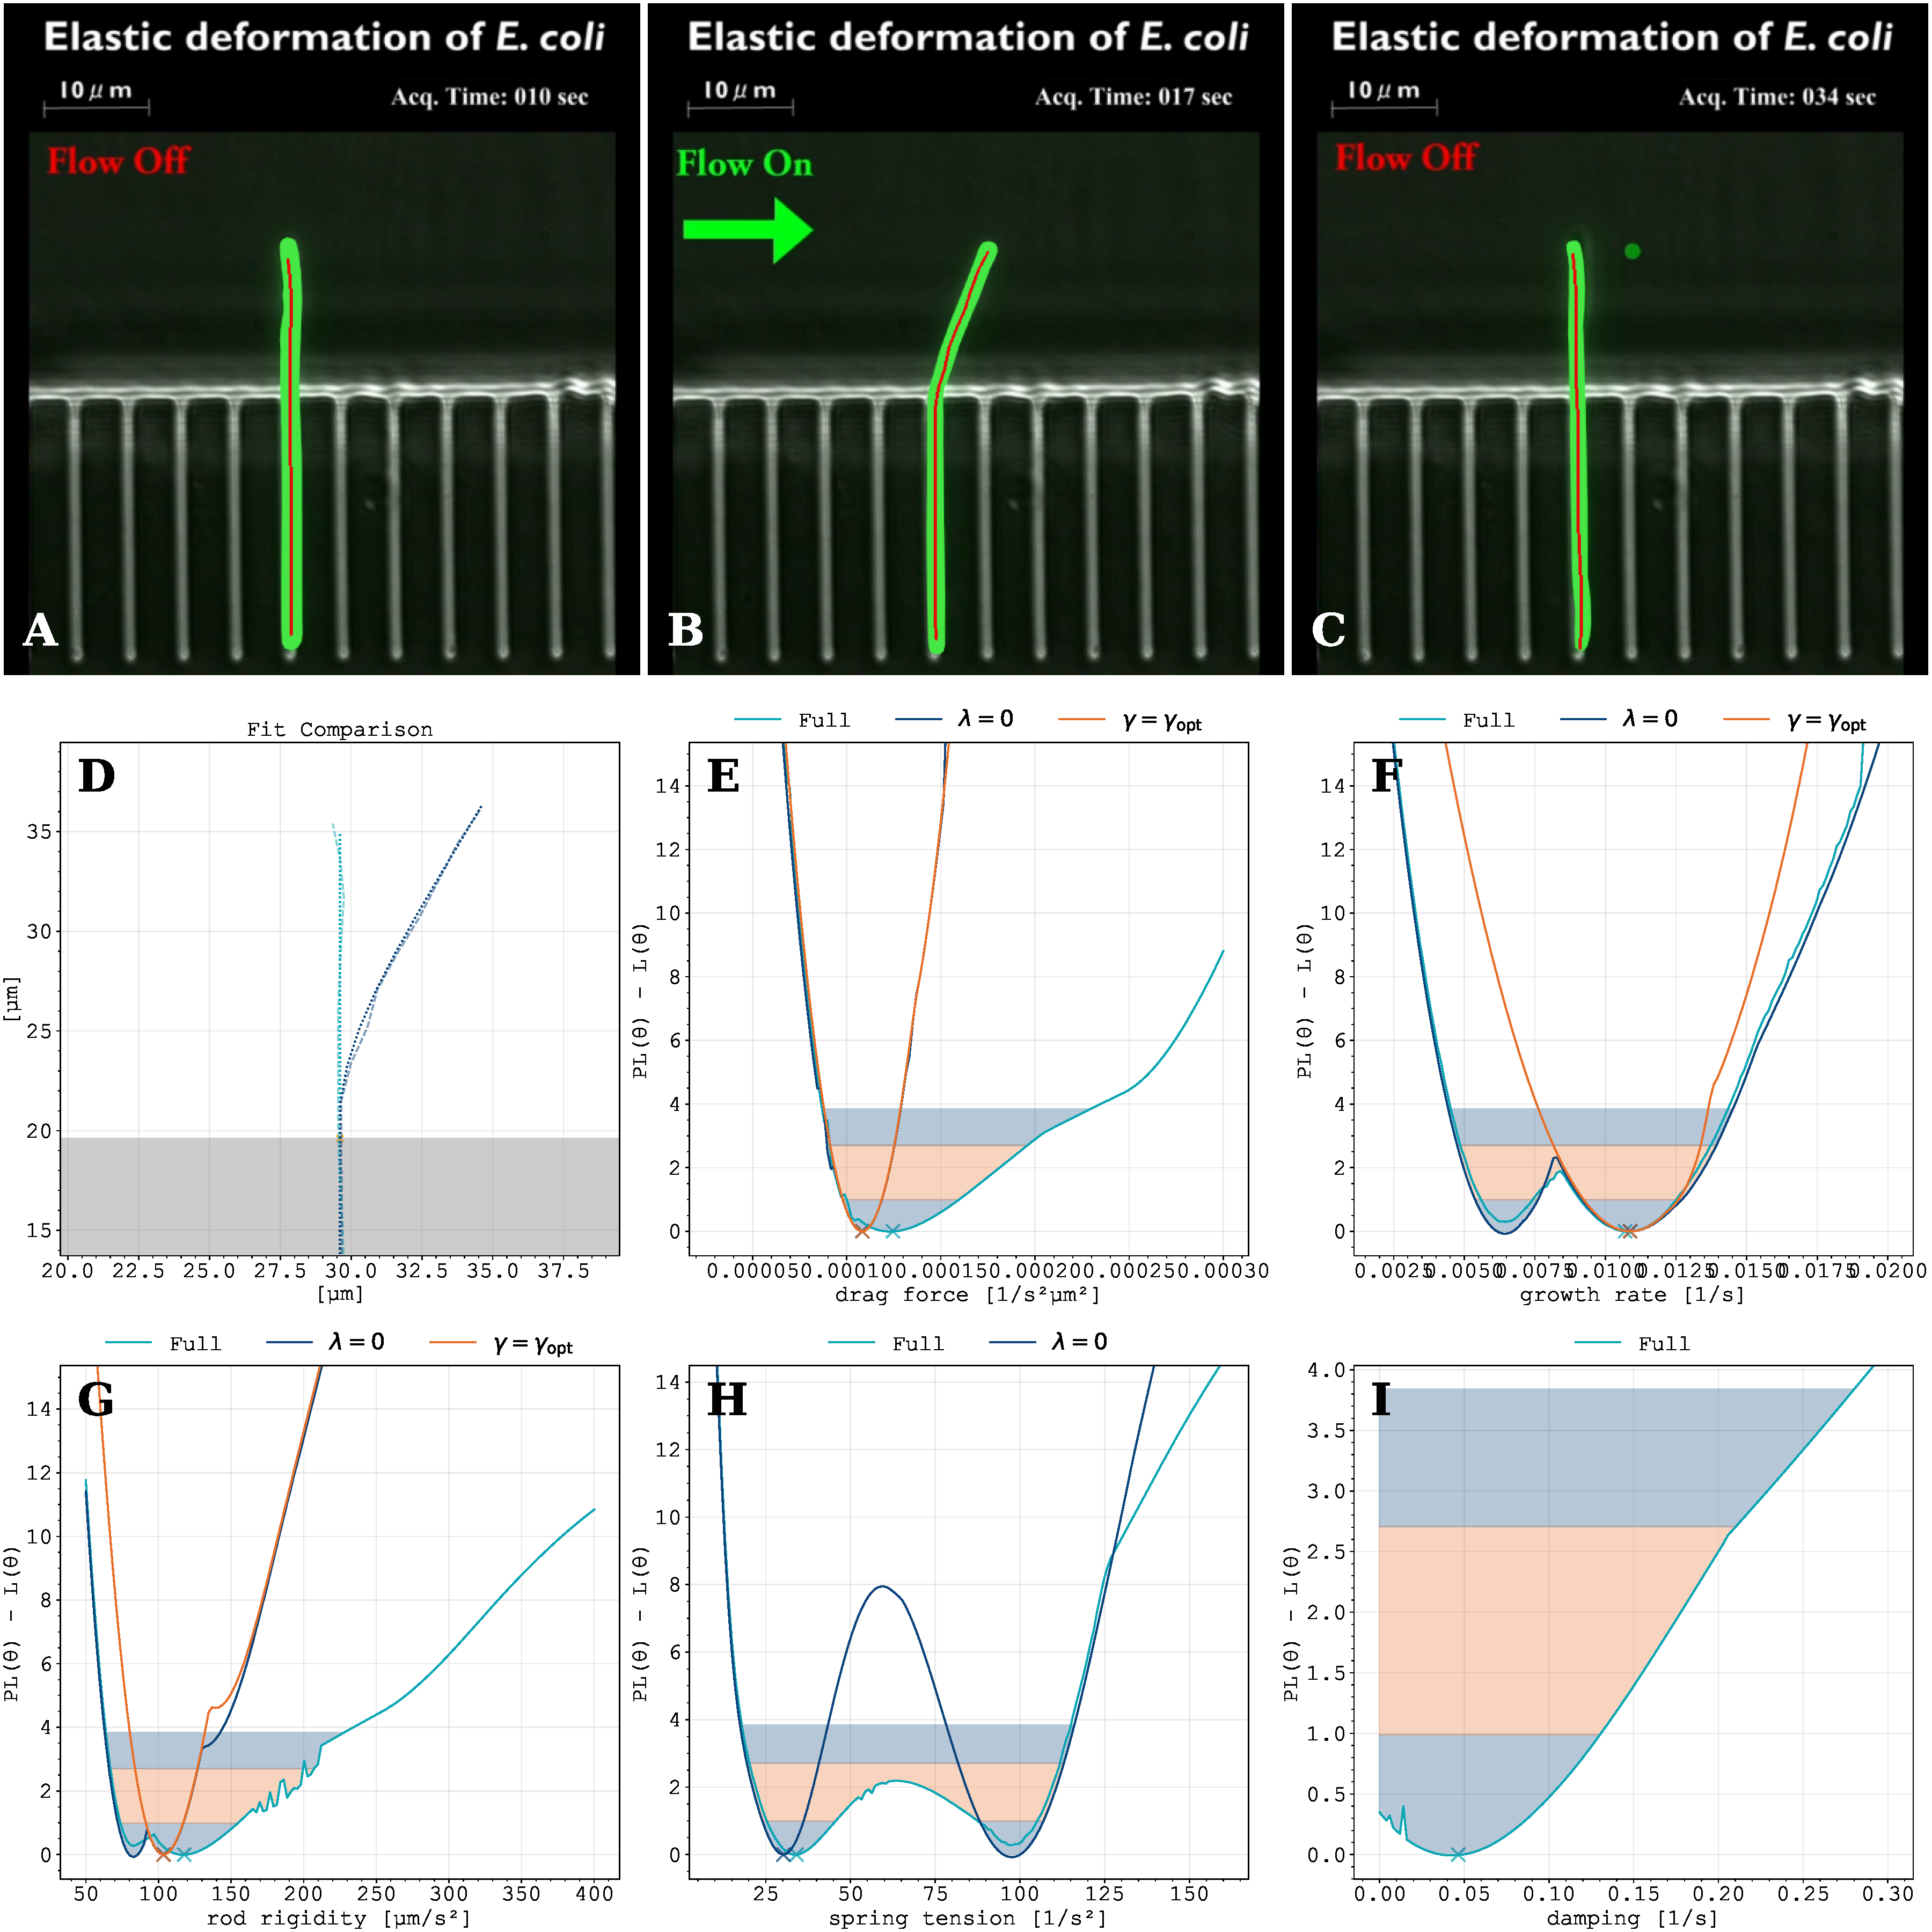
\includegraphics[width=\textwidth]{figures/crm_amir/profiles.pdf}
    \caption{
        (A-C) Manually segmented experimental snapshots of by Amir et al.~\cite{Amir2014_2}.
        The red line within the green mask shows the extracted position.
        (A-C) Snapshots of bending experiment by Amir et al.~\cite{Amir2014_2} with overlayed
        manual segmentation mask (bright green) and extracted position (red).
        The sequence shows the rod initially (A), under flow (B) and after relaxation (C).
        (D) Comparison of simulated and experimental rod in bent and relaxed state.
        (D-H) Profile-likelihoods for the estimated parameters.
        Bands of blue and yellow indicate confidence intervals of $68\,\%,90\,\%$ and $95\,\%$.
        Brigth blue curves represent the full model, dark blue a reduced model without damping
        $\lambda=0$ and orange curves when fixing the auxiliary spring tension parameter
        $\gamma=\gamma_\text{opt}$. {\bf [woher soll man denn den optimalen Parameter kennen?]} With these reductions, every parameter is identifiable.
    }
    \label{fig:amir-bending-simulation}
\end{figure}

%###################################################################################################
\subsection{Application 2: \acl{ecoli} growing on Agar}
\label{section:application-2}
In this section we study a collection of growing, dividing and physically interacting
\ac{ecoli}.
We consider two scenarios to apply the above developed metrics within a realistic context and
validate our approach.

Our dataset~\cite{Trude1982} consists of of a time-series of phase-contrast images (see
Figure~\ref{fig:application-2-data-overview} (A)).
We segmented them using the omnipose toolkit~\cite{Cutler2022} (see
Figure~\ref{fig:application-2-data-overview} (B)) and extracted their trajectories with the
previously described pipeline (Section~\ref{sec:supplement-extraction-algorithm}).
The model is initialized with the extracted position of the first snapshot and parameters are
optimized to minimize the respective metrics.

For our first case-study, we select 7 individual images spanning over an interval of
$\SI{20}{\minute}$ without any division events.
Figure~\ref{fig:application-2-data-overview} (C) displays the initial (left) an intermediate
(middle) and final state of this interval.
From these images we can already see that the cellular growth is the driving factor behind the
dynamics of the system.
We estimate the parameters of this systems via the direct position-space metric
(see Section~\ref{subsec:direct-metric}).

In the second case-study, we extend the interval to $\SI{85}{\minute}$ whith 13 images including
division events.
This requires the use of the Lineage-aware image-space metric (see
Section~\ref{subsec:image-space-metric}).

\begin{figure}[H]
    \centering
    \begin{tikzonimage}[width=0.49\textwidth]
        {figures/data/crm_fit/001044.png}%
        \node at (0.02, 0.98)[anchor=north west, white]{\textbf{A}};
    \end{tikzonimage}%
    \hspace{0.01\textwidth}%
    \begin{tikzonimage}[width=0.49\textwidth]
        {figures/data/crm_fit/001044-markers.pdf}%
        \node at (0.02, 0.98)[anchor=north west, white]{\textbf{B}};
    \end{tikzonimage}\\
    \vspace{0.01\textwidth}%
    \begin{tikzonimage}[width=0.28\textwidth]
        {figures/crm_fit-data-progression.png}
        \node at (0.02, 0.98)[anchor=north west, white]{\textbf{C}};
    \end{tikzonimage}%
    \hspace{0.01\textwidth}%
    % TODO Use matplotlib to combine plots
    \begin{tikzonimage}[width=0.35\textwidth]
        {figures/crm_estimate_params/IWF-Goettingen/positions/rod-lengths-individual.pdf}%
        \node at (0, 1)[anchor=north west, black]{\textbf{D}};
    \end{tikzonimage}%
    \begin{tikzonimage}[width=0.35\textwidth]
        {figures/crm_estimate_params/IWF-Goettingen/positions/growth-rates-bar-plot.pdf}%
        \node at (0, 1)[anchor=north west, black]{\textbf{E}};
    \end{tikzonimage}%
    \caption{
        (A) Snapshot of initial microscopic images.
        (B) Segmentation result of (A).
        (C) Initial (left), intermediate (middle) and final (right) microscopic snapshots.
        A complete list of snapshots is included in the supplementary material (see
        \nameref{sec:supplement-data-details}).
        (D) Analysis of growth for the chosen time interval.
        (E) The histogram of the growth parameters exhibit significant cell-cell variability.
        % The obtained results are further discussed in the supplementary material
        % (Section~\ref{sec:supplement-reuse-estimated-parameters}).
    }
    \label{fig:application-2-data-overview}
\end{figure}


\paragraph{Cell-Cell Variability within the Dataset}
\label{paragraph:parameter-estimation-individual-treatment}

As discussed in Section~\ref{sec:role-of-heterogeneity}, in order to properly estimate the
parameters of our system, we need to account for natural cell variability, thus assigning optimized
parameters on a per-cell basis.
Figure~\ref{fig:application-2-data-overview} (D) shows the length of the rods as determined via our
extraction algorithm (solid curves).
To quantify this heterogeneity, we fit the individual curves with an exponential:
\begin{equation}
    l(t) = l_0 \exp(\mu t).
    \label{eq:exponential-growth-model}
\end{equation}
where $l_0$ is the starting length of the rod and $\mu$ is the growth rate.
Figure~\ref{fig:application-2-data-overview} (E) shows the histogram of the obtained growth rates.
The distinct phenotypic properties of the cells result in large deviations of the individual growth
rates.
These results show that one needs to account for cell-cell variability by referring to cell-specific
growth parameters.

% --------------------------------------------------------------------------------------------------
\subsubsection{Without Division}
\label{sec:application-1-without-division}
First, we restrict our analysis to an time interval of $\SI{20}{\minute}$ without any cell division
events, which enables us to use the computationally more efficient direct position-space metric
(Section~\ref{subsec:image-space-metric}).
Using our complete mechanical model (Section~\ref{sec:computational-model}), we optimized a total
of $11$ parameters: $5$ global parameters that govern mechanics and interactions (damping
$\lambda$, radius $R$, and parameters $n,m,V_0$ of the mie potential) together with $6$
cell-specific growth rates $\mu_i$.
\ac{ecoli} are short and typically straight, allowing us to fix the rigidity $\eta$ to a high value.
The spring constant exerts a force parallel to the connecting segment between two vertices.
In the presented scenario forces which actively extend the rod are negligible.
Therefore, the spring tension in combination with a damping effect merely ensures that the length of
the rod is maintained.
For this reason, we do not expect to be able to properly estimate the value of this parameter and
therefore assume a high fixed value such that the rod length is maintained.

We employed a two-stage optimization strategy.
First, the parameter space was explored using a global Differential Evolution
algorithm~\cite{Storn1997} which was seeded using Latin-Hypercube sampling~\cite{McKay1979}.
Finally, local minimization was performed using the L-BFGS-B algorithm~\cite{Liu1989}.

Figure~\ref{fig:parameter-estimation-optimized-results} (A-B) shows differences between the
numerical results using the optimized parameters and experimental data of the final time step in two
distinct ways.
By visually inspecting these subfigures, we can already see that the numerical results match closely
to the provided data.
However, in order to systematically analyze these differences and investigate if the obtained
parameters could be identified, we employ the \textit{profile-likelihood} method.

Figure~\ref{fig:parameter-estimates-single-step} shows the profile-likelihoods for each optimized
parameter.
In total, we compare four distinct models, covering both Morse and Mie-type interactions with and
without a fixed damping constant $\lambda=\SI{1}{\per\minute}$.
Figure~\ref{fig:parameter-estimates-single-step} (A) displays the \textit{profile-likelihood} for
the damping constant $\lambda$ of the non-reduced models.
It exhibits a wide range of permissible parameter values which suggests a possible reduction of our
model.
However, we can not simply omit this parameter by effectively setting it to zero as the profile
shows a steep ascend for $\lambda\rightarrow0$ which means that the observed results would be
incompatible with this choice.
Therfore, we assign a fixed value for this parameter.

The parameters which characterize the Morse-type interaction are the potential stiffness $\omega$,
strength $V_0$ and radius $R$, Figure~\ref{fig:parameter-estimates-single-step} (B, E, F).
While the potential stiffness (B) and radius (F) can be accurately estimated from the given data,
the potential strength (E) is subject to a practical unidentifiability~\cite{Raue2009} which is
resolved by fixing the damping constant to $\lambda=\SI{1}{\per\minute}$.
The Mie potential uses two parameters $n,m$ (C,D) to determine the shape of the interaction
potential which allows it to describe a larger class of curves.
However, as the profile-likelihoods presented in Figure~\ref{fig:parameter-estimates-single-step}
(A,C,D,E) show, that the exponents $n,m$ of the Mie-type interaction can not be estimated, even when
reducing the model via $\lambda=\SI{1}{\per\minute}$.
It is necessary to enhance the data set, e.g., by including additional scenes showcasing a greater
variety of interactions in order to remove this practical non-identifiability.
We further note that the two interaction types result in different predictions for the radii
(Figure~\ref{fig:parameter-estimates-single-step} (F)).
However, their $68\,\%$ confidence intervals overlap.
Figure~\ref{fig:parameter-estimates-single-step} (G-L) show that the growth rates can be estimated
for any interaction type but the Mie-type interaction shows wider confidence intervals and thus
greater uncertainty in the predicted parameter value.

\begin{figure}[H]
    \centering
    \begin{tikzonimage}[width=0.49\textwidth]
        {figures/crm_fit/morse_partial/snapshots/predicted-006562.png}%
        \node at (0.025, 0.975)[anchor=north west, white]{\textbf{A}};
    \end{tikzonimage}%
    \hspace{0.01\textwidth}%
    \begin{tikzonimage}[width=0.49\textwidth]
        {figures/crm_fit/morse_partial/celldiffs/diff-006667.png}%
        \node at (0.025, 0.975)[anchor=north west, white]{\textbf{B}};
    \end{tikzonimage}%
    \caption{
        Predicted results by the reduced model with Morse-type interaction.
        (A) Final microscopic image of the time series with the predicted positions and cell
        envelopes overlayed on top.
        The numerically simulated results neatly match the biological reality and possible
        differences can not be seen directly.
        Therefore subfigure (B) showcases these differences by utilizing the developed methods of
        the image-space metric.
        Note that this is done purely for visualization and not for optimization of the system.
    }
    \label{fig:parameter-estimation-optimized-results}
\end{figure}

\begin{figure}[H]
    \centering
    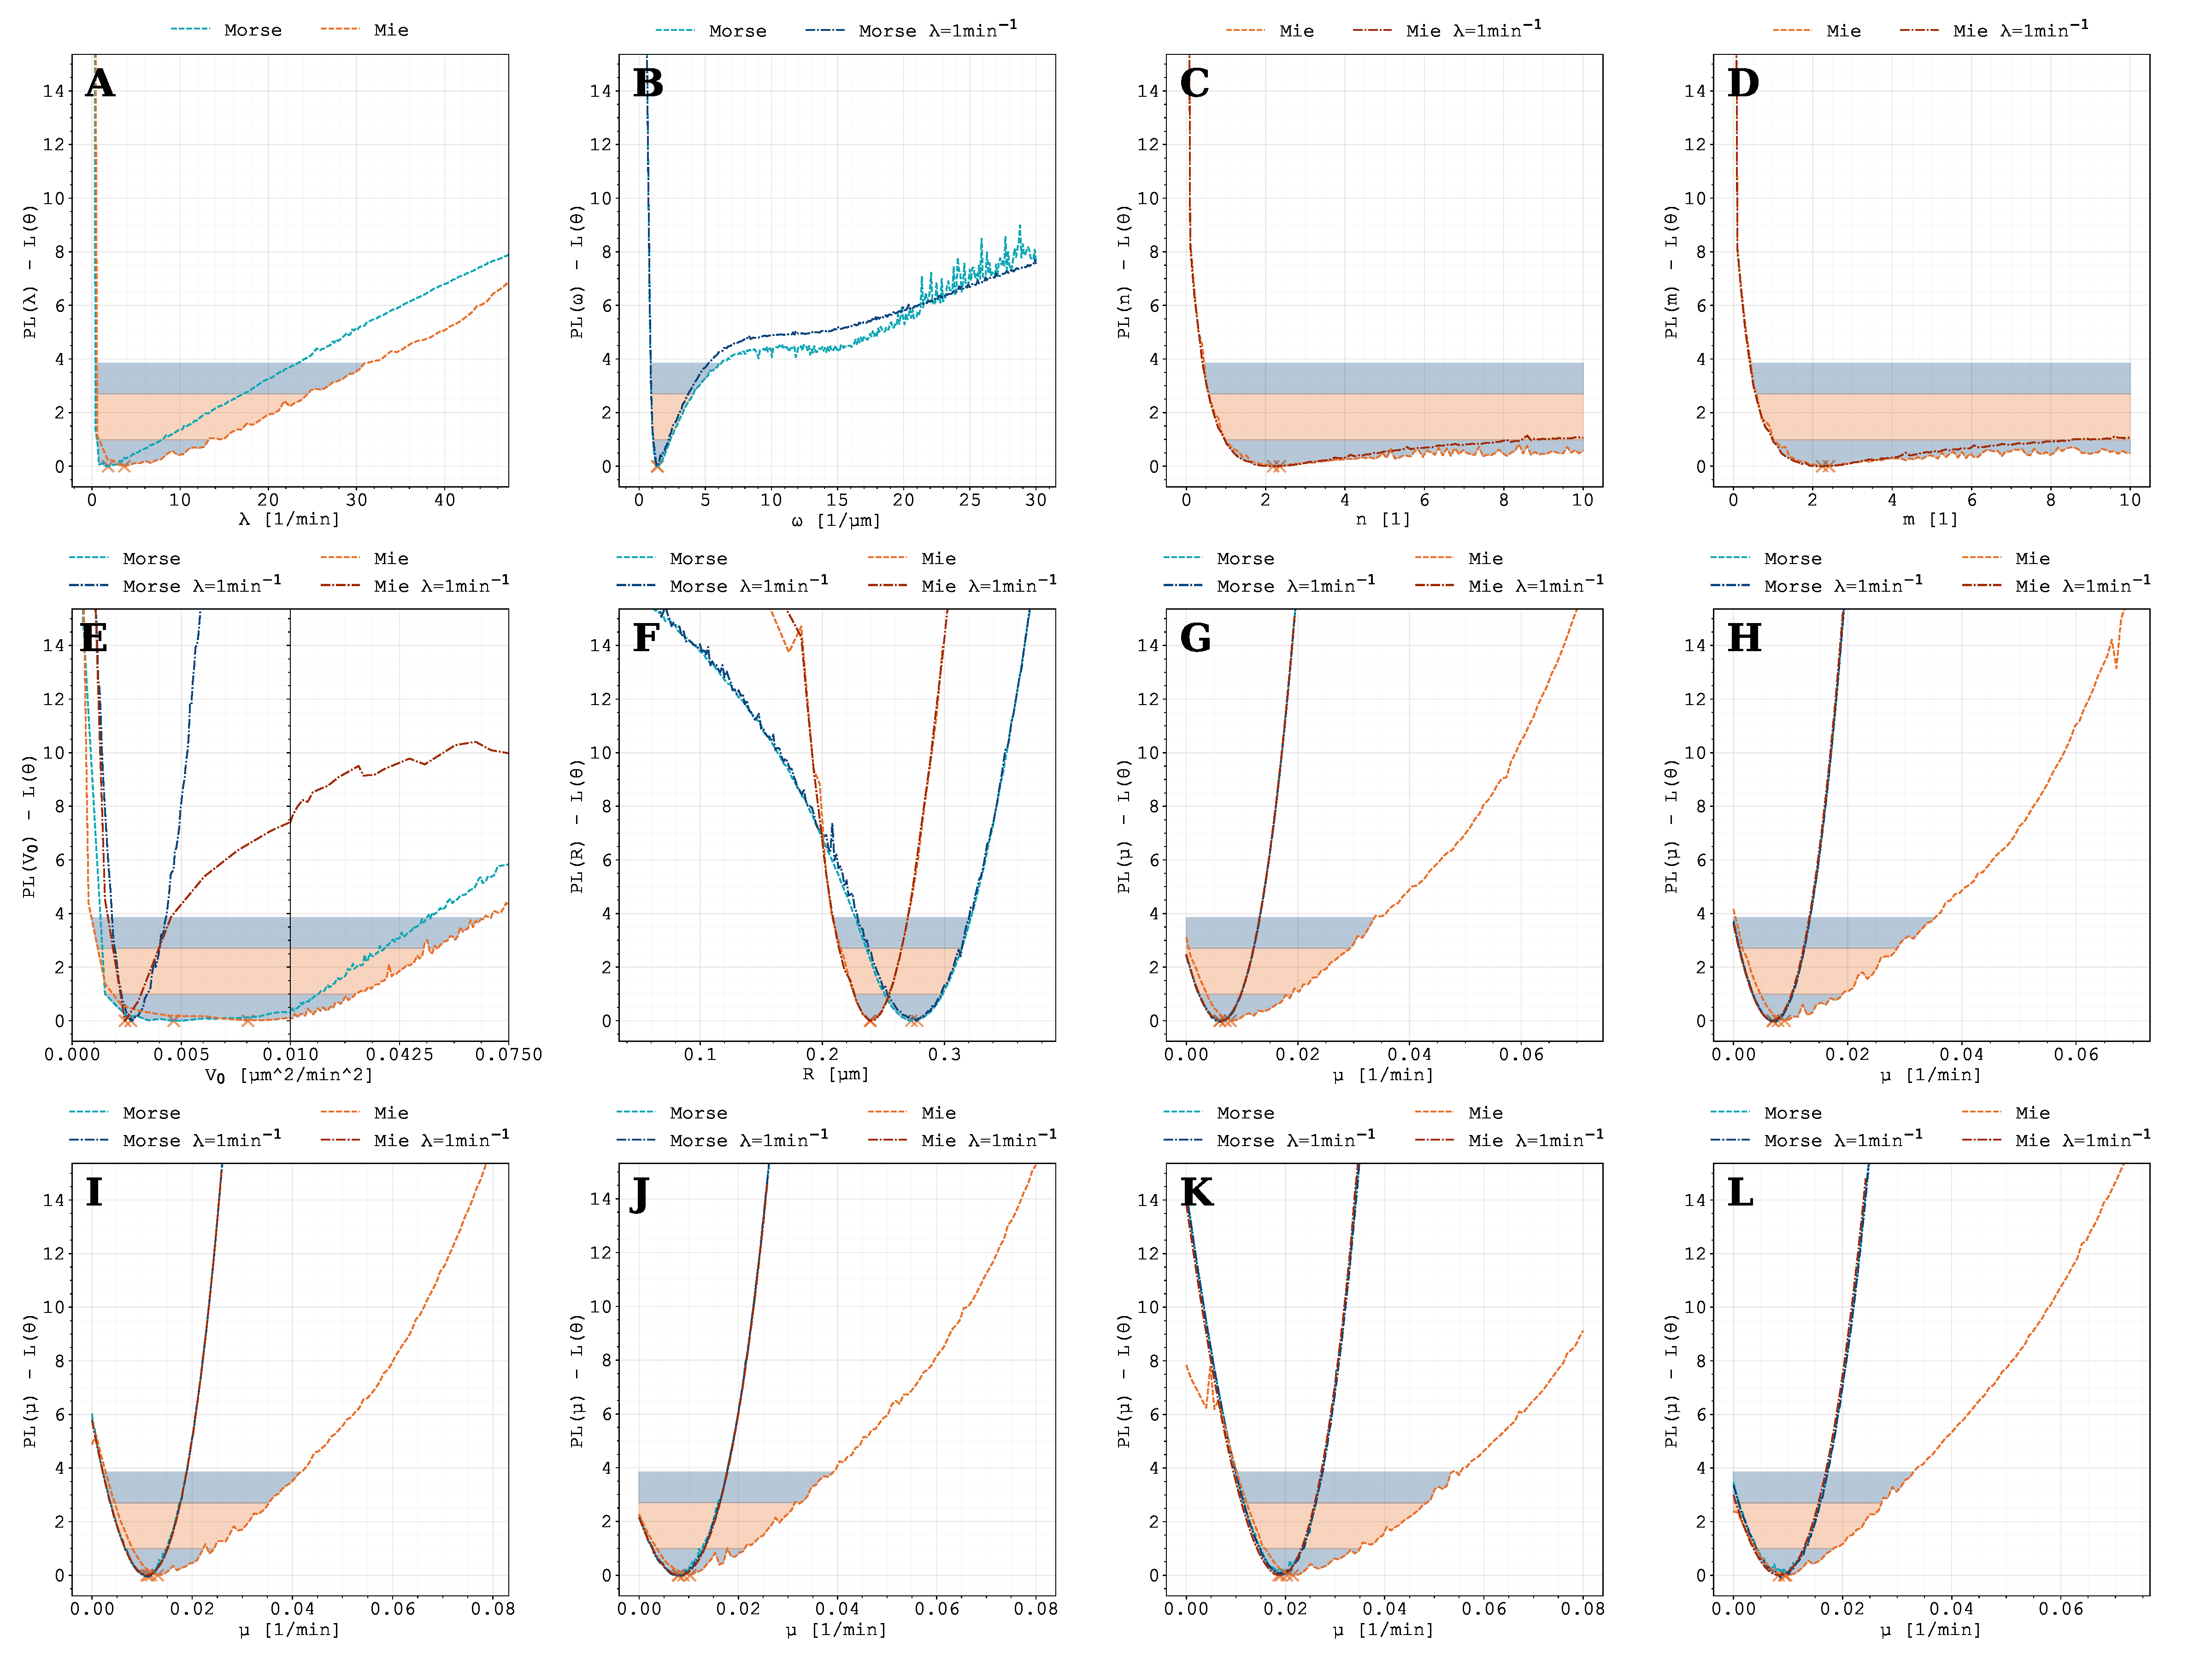
\includegraphics[width=\textwidth]{figures/crm_fit/profiles-all.pdf}
    \caption{
        (A-L) Likelihood profiles for 4 scenarios: Full and reduced model, by setting the damping
        constant to $\lambda=\SI{1}{\per\minute}$, with Morse/Mie interaction.
        Blue and yellow bands represent confidence intervals of $68\,\%,90\,\%$ and $95\,\%$,
        respectively.
        (A) Damping constant before model reduction.
        (B) Potential Stiffness $\omega$ of the Morse potential.
        (C-D) Exponents $n,m$ of the Mie potential.
        (E) Strength $V_0$ of the interaction potential.
        The x-axis is split in the middle to display a narrow and wider range for lower and higher
        parameter values.
        (F) Radius $R$ (thickness of the rod) of the potential.
        (G-L) Individual growth rates $\mu$ of the 6 bacterial agents.
    }
    \label{fig:parameter-estimates-single-step}
\end{figure}

% --------------------------------------------------------------------------------------------------
\subsubsection{With Division}
\label{sec:application-1-with-division}
In the next step, we extend the analyzed time interval to $\SI{85}{\minute}$, which includes cell
division events.
This requires us to use the Lineage-aware Image-Space Metric
(section~\ref{section:parameter-estimation}).
A practical challenge in extending the time series arose during data preparation: the segmentation
algorithm was not able to properly label the individual bacteria for timepoints close to division
events.
This effect is frequently observed and in segmentation tasks and presents a challenge in the
parameter estimation process.
One possible solution would be to manually segment the image which is often done in practice.
However, in order to show that the combination of our model and analysis techniques is able to deal
with these common practical limitations, we omit the subset of snapshots surrounding the division
events, leaving us with incomplete temporal data.
Such a robustness with respect to the incompleteness of data is of utmost importance for any
automated approach involving our methods.

In order to compare experimental and simulation results via the Lineage-aware Image-space metric,
there are four required steps which are executed within any single optimization iteration.
Firstly, results need to be generated by performing the simulation.
Afterwards, the corresponding masks is generated and then adjusted in such a way that it can be
compared directly with experimental cell masks.
This requires us to map the cell-lineage of the numerical result to the experimental data.
Finally, we use the previously established Lineage-aware image-based metric for the comparison.

% Since we have already optimized said system, we can reduce the computational demand by choosing the
% parameters which were obtained by our previous attempts and extend them with the parameters that the
% daughter cells will carry.
In addition to the previously used parameters, we also need to estimate division lengths at
which the bacteria split and the new individual growth rates of the daughter cells as additional
parameters.
Since our simulation involves the division of 4 cells into 8 new ones, this amounts to a total of
$4$ division lengths and $8$ new growth rates .
% But to decrease the size of the parameter space, we assume that the growth rates of the daughter
% cells are identical between every sibling, leaving us at only $4$ new growth rates and a total of
% $8$ parameters.
% Future approaches should aim to loosen this assumption, allowing to optimize every new growth rate.
To optimize this system, we used a similar optimization approach by again seeding with samples
generated via Latin-Hypercube~\cite{McKay1979}, then applying the differential evolution
algorithm~\cite{Storn1997} and finally a local minimization with Nelder-Mead~\cite{Gao2010}.
We used the value $p_p=0.5$ for the parent penalty, which aims to provide a smooth transition
between not accounting for parental relationships, i.e. $p_p=0$ and assigning full weighting, i.e.
$p_p=1$.
Figure~\ref{fig:celldiffs-progression-with-division} shows the difference between the cell mask as
given by the data and the cell mask predicted by the best fit of our model.
As expected, the fully-optimized system does not produce differences where the parental penalty is
required.
However, this approach is still frequently used within the the optimization scheme itself and aids
in smoothing the calculation of gradients between distinct results.

% We can again calculate likelihood profiles for every optimized parameter.
Since further mathematical analysis is required to assess how to utilize the Lineage-aware
Image-Space metric for maximum-likelihood approaches, we simply display profiles of the cost
function when fixing a single parameter and reoptimizing the remaining ones.
While only confidence bands for likelihood profiles as presented in the previous sections could
paint a clearer picture with regards to the identifiability of the parameters, we can still
identify some trends.

We used the Morse potential as an interaction type since we have already seen in the preceding
section that the mie potential could not be identified properly.
The profiles in Figure~\ref{fig:likelihood-profiles-comparison-with-division} show that every
parameter can be identified from the given data.
The individual subplots show 3 curves containing the metric used for comparison, the same metric
when removing contributions of the calculated overlaps and when setting the parent penalty $p_p=1$,
thus ignoring these contributions.
In particular, all interaction parameters such as the potential stiffness, strength and radius
(A,B,C) are well bound from below and above.
The potential stiffness is particularly influenced by contributions from overlaps, which well
explicable since higher parameter values result in a steeper potential curve, thus beeing less
permissible to overlapping radii.
The profiles of the growth rates of cells (0-4) which lead to a division event, exhibit a stark
negative peak which indicates good identifiability of these parameters.
In contrast, the profiles of growth rates of cells (5,6) which do not divide during the time
interval are less pronounced.
The division lengths of the dividing cells (0-4) also show a clear negative dip, thus enabling a
proper estimation this parameter.
All growth rates for the daughter cells (M-T) show similar behaviour to the
non-dividing cells which are present at the initial state.
Their profiles indicate that a optimum was achieved and significantly increase with higher values
while being less stringently bound from below.

We can clearly see the effect of the parent-penalty in all parameters related to growth and
division.
It is a matter of future studies to further explore how this treatment can affect the optimization
scheme and the values of the obtained parameters.

Coming back to the lack of data around the division event, our results show that despite this
incompleteness, our model is still able to determine the respective parameters such as division
lengths and growth rates of cells (0-4) accurately.
In particular, it exhibits not plateaus due to missing data points.
This phenomon can be attributed to our mechanistic understanding of the problem and would not have
been possible by other approaches such as purely statistical models.
{\bf [diesen Abschnitt muss ich nochmals genau lesen, wenn wir über den Rest diskutiert haben]}
\begin{figure}[H]
    \centering
    \begin{tikzonimage}[width=0.32\textwidth]
        {figures/crm_divide/masks_diff/000000.png}%
        \node at (0.025, 0.975)[anchor=north west, white]{\textbf{A}};
    \end{tikzonimage}%
    \hspace{0.01\textwidth}%
    \begin{tikzonimage}[width=0.32\textwidth]
        {figures/crm_divide/masks_diff/000010.png}%
        \node at (0.025, 0.975)[anchor=north west, white]{\textbf{B}};
    \end{tikzonimage}%
    \hspace{0.01\textwidth}%
    \begin{tikzonimage}[width=0.32\textwidth]
        {figures/crm_divide/masks_diff/000020.png}%
        \node at (0.025, 0.975)[anchor=north west, white]{\textbf{C}};
    \end{tikzonimage}%
    \caption{
        Snapshots of differences between cell masks obtained from the data and predicted by the best
        fit of our model at (A) the beginning (B) right before the division event (C) right after
        the division event.
        The optimization routine was able to fully mitigate the cost assigned due to parental
        relationships which means that the fully-optimized result contains division lengths that
        match the data.
    }
    \label{fig:celldiffs-progression-with-division}
\end{figure}

\begin{figure}[H]
    \centering
    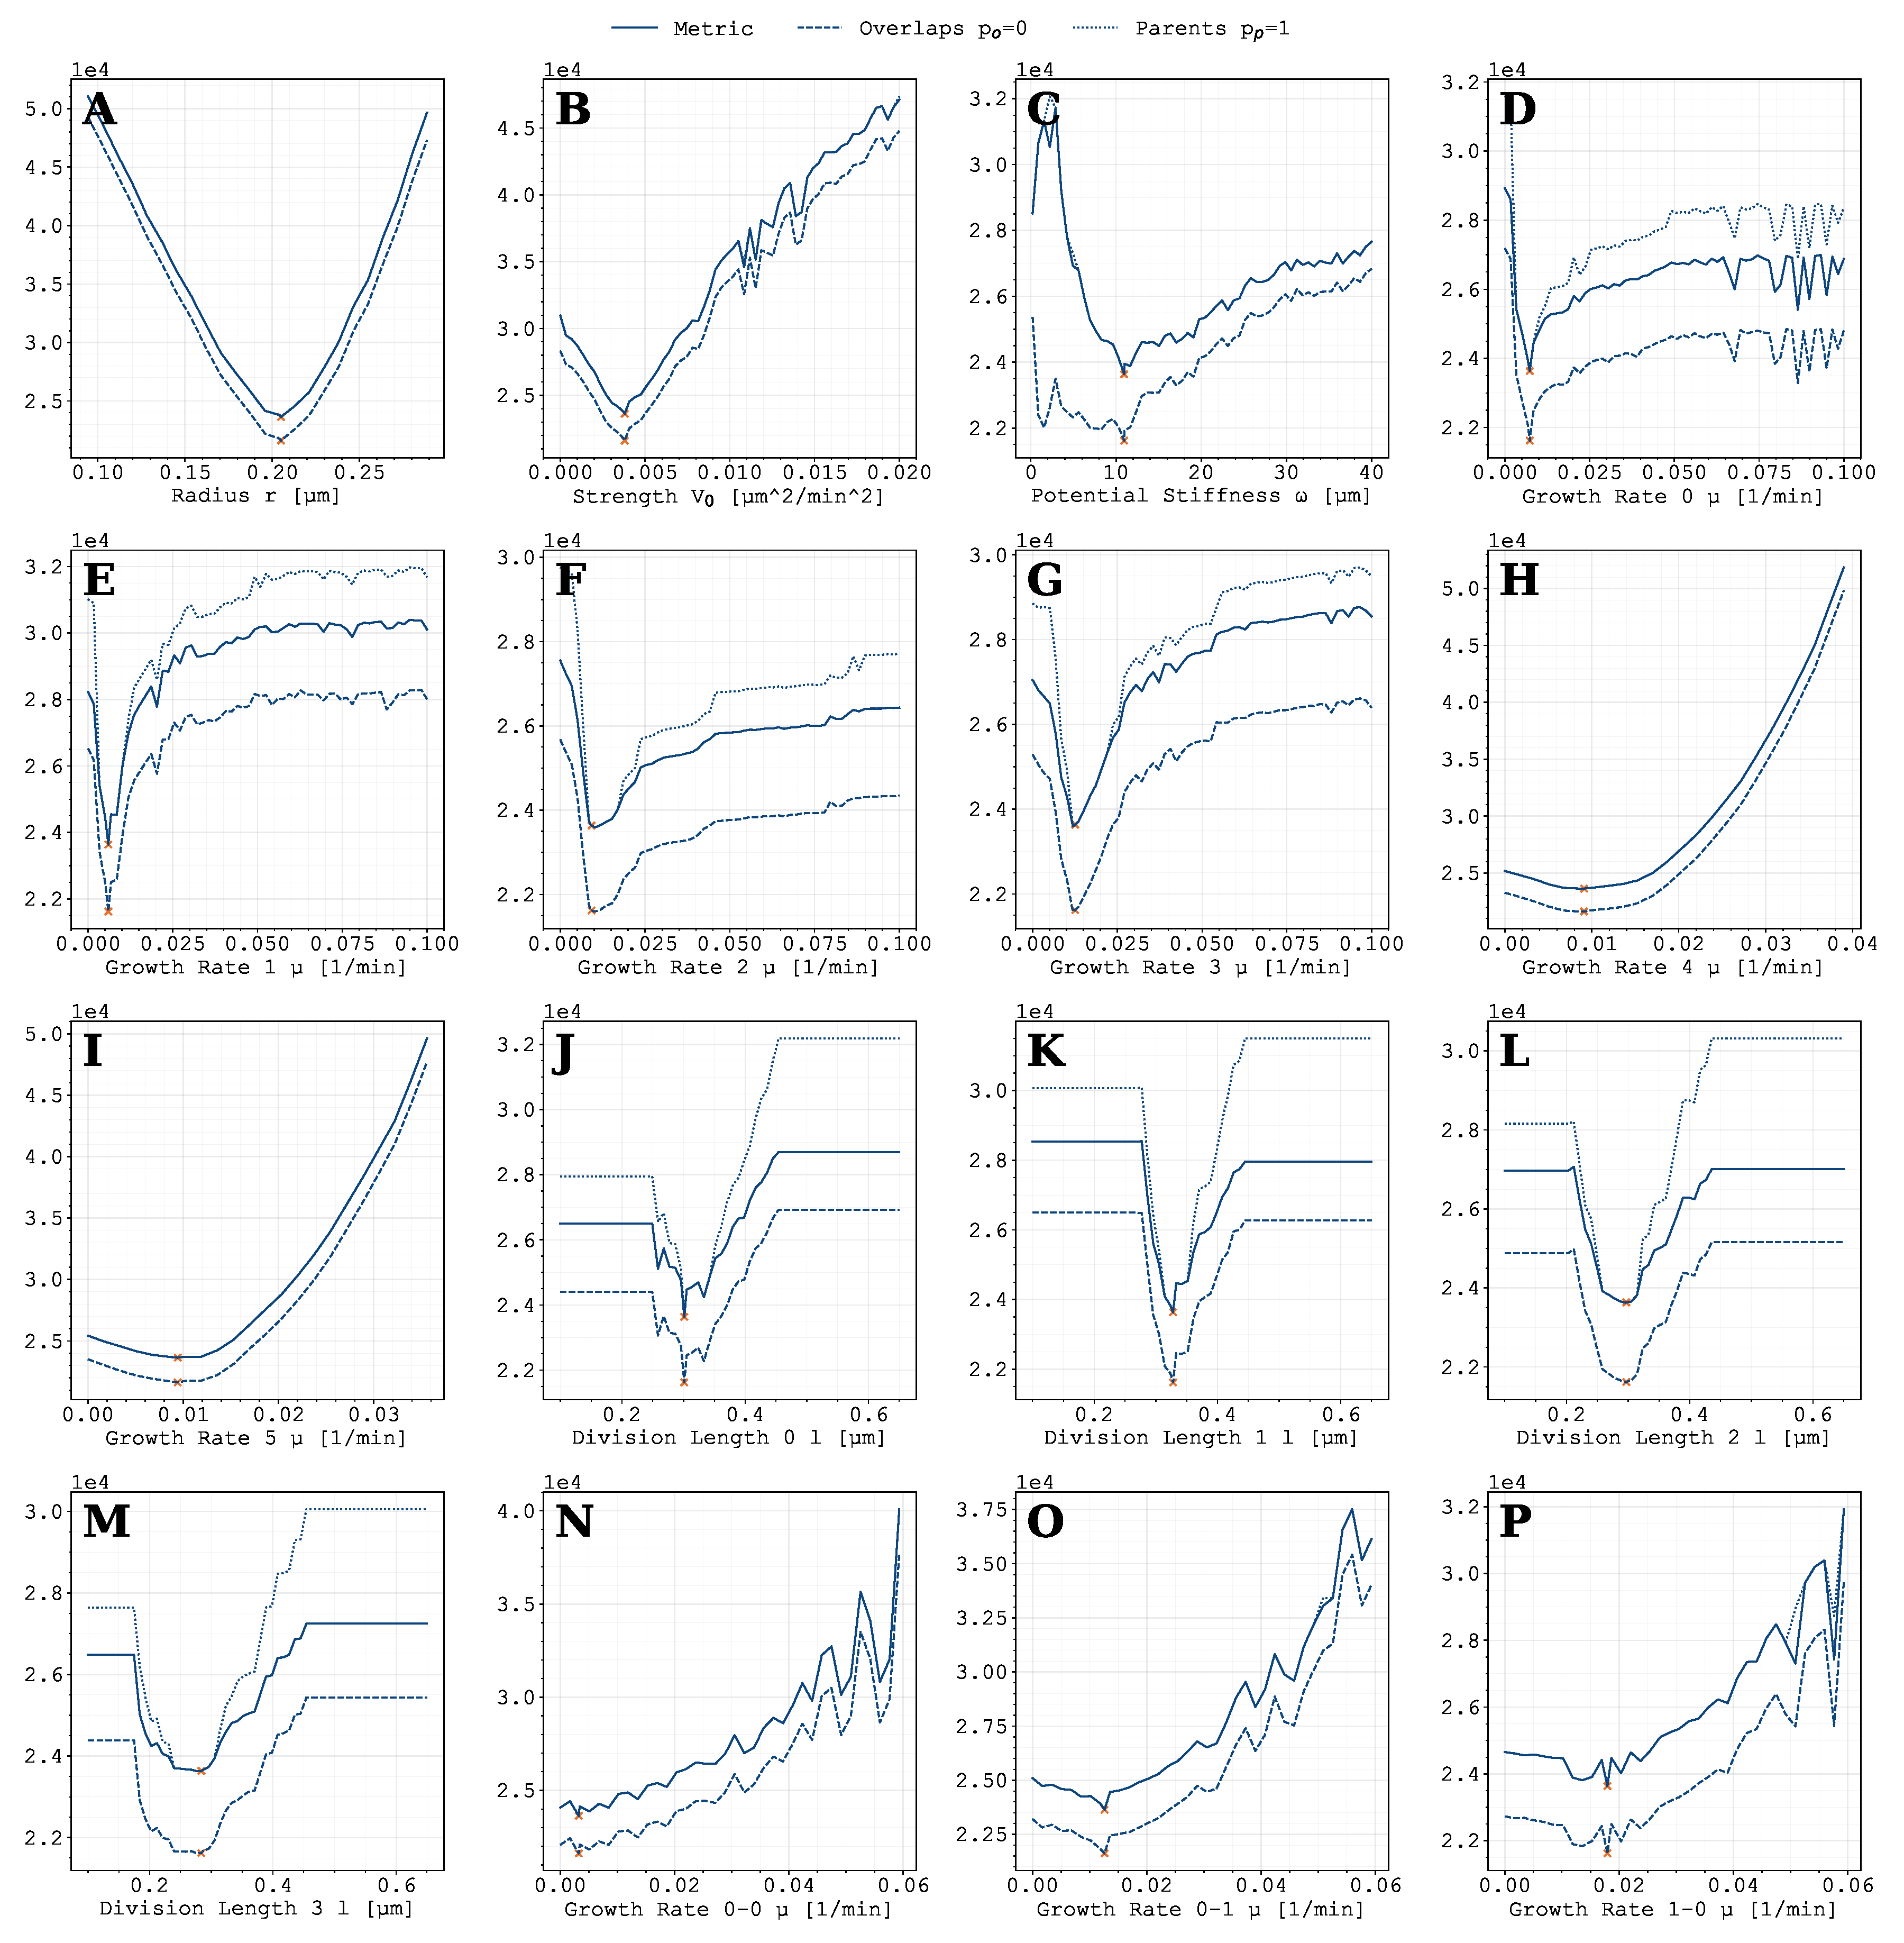
\includegraphics[width=\textwidth]{figures/crm_divide/profiles-1.pdf}
    \caption{
        Profiles of optimized cost functions when scanning along one parameter axis.
        (A) Potential Stiffness (B) Strength (C) Radius of the Morse Potential.
        (D-G) Growth rates of mother cells and (H,I) non-dividing cells.
        (J-M) Division lengths of the mother cells.
        (N-P) Growth rates of daughter cells.
        For brevity, we display the remaining growth rates of the daughter cells in the
        supplementary material Figure~\ref{fig:supplement-profiles-with-division}.
    }
    \label{fig:likelihood-profiles-comparison-with-division}
\end{figure}

\subsubsection{Comparison of Estimated Parameters}
In this section, we compare the estimated parameter values of the various approaches that we have used.
It is important to keep in mind that the ground truth differs from the first part (without cell
division) to the second part (with cell division).
Furthermore, both approaches involve additional steps when determining the overall growth of the
bacteria.
The direct approach utilizes the positions of the cells which involves their extraction via our
developed algorithm.
The Lineage-aware Image-Space metric utilizes only the masks of the data and thus involves one step
less in the preprocessing steps.
These differences may influence the optimized parameter values.

Table~\ref{tab:comparison-growth-rates} shows the obtained values for the growth rates via the
different techniques.
The first part lists growth rates determined by direct analysis from the data (Data Extraction).
As discussed before, growth rates can be determined by either fitting the exponential growth model
(equation \ref{eq:exponential-growth-model}) to the extracted positions (Position Fit) or directly
to the count of pixels of the associated instance-level segmentation mask of the cell (Pixel Fit).
We see that the two methods lead to significant differences between the numerical values.

The next parts contain the results of section~\ref{sec:application-1-with-division} and
\ref{sec:application-1-without-division} including growth rates of the resulting daughter cells.
One clear trend within the direct position-space comparison block is the ordering of growth rates.
The cells with largest to lowest growth rate are 4,2,3,5,1,0 where the order is only violated in
the first case, switching between 3 and 5 which is not surprising due to their similarity in
numerical values.
However this trend is not picked up when estimating parameters with the Lineage-aware Image-Space
metric.

Finally, the table lists the total division lengths $\tilde{l}=(n_\text{vertices}-1)l$ which is the
estimated total length at which the mother cell has divided.

\begin{table}[H]
    \centering
    % \textbf{Growth Parameters obtained by various Methods}
    \begin{tabular}{l c c c c c c}
        % \multicolumn{7}{l}{}\\
        \multicolumn{7}{c}{Estimated Growth Rates $[\mu]=\SI{}{\per\minute}$}\\
        \toprule
        \textbf{Data Extraction} & Cell $0$ & Cell $1$ & Cell $2$ & Cell $3$ & Cell $4$ & Cell $5$\\
        \midrule
        Position Fit & 0.0069 & 0.0054 & 0.0115 & 0.0076 & 0.0103 & 0.0084\\
        Pixel Fit    & 0.0062 & 0.0068 & 0.0034 & 0.0071 & 0.0018 & 0.0059 \vspace{0.2cm}\\
        \multicolumn{7}{l}{\textbf{Direct Position-Space Metric}}\\
        \midrule
        Mie                                 & 0.0079 & 0.0090 & 0.0131 & 0.0103 & 0.0215 & 0.0097\\
        Mie $\lambda=\SI{1}{\per\minute}$   & 0.0060 & 0.0069 & 0.0109 & 0.0080 & 0.0186 & 0.0083\\
        Morse                               & 0.0070 & 0.0078 & 0.0118 & 0.0089 & 0.0203 & 0.0094\\
        Morse $\lambda=\SI{1}{\per\minute}$ & 0.0060 & 0.0070 & 0.0113 & 0.0078 & 0.0191 & 0.0093 \vspace{0.2cm}\\

        \multicolumn{7}{l}{\textbf{Lineage-aware Image-Space Metric} (Morse $\lambda=\SI{1}{\per\minute}$)}\\
        \midrule
        Mother                              & 0.0073 & 0.0060 & 0.0092 & 0.0126 & 0.0091 & 0.0094\\
        Daughter                            & 0.0032 & 0.0179 & 0.0052 & 0.0185 & - & -\\
        Daughter                            & 0.0126 & 0.0048 & 0.0011 & 0.0005 & - & -\\
        Division Lengths $[\tilde{l}]=\unit{\micro\metre}$
                                            & 2.1080 & 2.2957 & 2.0803 & 1.9870\\
        \bottomrule
    \end{tabular}
    \caption{
        Growth rates and division lengths calculated by the distinct approaches explained in the
        text.
        This includes growth rates of the daughter cells and total division lengths $\tilde{l}$ of
        the mother cells.
    }
    \label{tab:comparison-growth-rates}
\end{table}

While growth rates can be directly compared between the various approaches, the same cannot easily
be done with the remaining kinetic parameters which are listed in
Table~\ref{tab:comparison-kinetic-parameters}.
This is because the type of interaction potential greatly determines the values of these parameters.
Parameters such as the exponents $n,m$, or the potential stiffness $\omega$, influence the overall
magnitude of the potential, thus also influencing the strength $V_0$.
However, one clear effect can be seen when comparing the potential stiffness $\omega$ of the direct
approaches with the Imaging results.
Due to the fact that the Image-Space metric penalizes overlapping regions of cells, the potential
stiffness is much larger.
This could also explain the lower radius value compared to the other results.

\begin{table}[H]
    \centering
    \begin{tabular}{l c c c c}
        \multicolumn{5}{c}{Estimated Kinetic Parameters}\\
        \toprule
        \makecell[l]{\\\textbf{Direct}}
            & \makecell{Damping\\$[\lambda]=\unit{\per\minute}$}
            & \makecell{Exponents $n,m$/\\Stiffness $[\omega]=\unit{\per\micro\metre}$}
            & \makecell{Strength\\$[V_0]=\unit{\micro\metre^2\per\minute^2}$}
            & \makecell{Radius\\$[r]=\unit{\micro\metre}$}\\
        \midrule
        Mie                         & 3.670 & 2.358, 2.408 & 0.0081 & 0.239\\
        Mie $\lambda=\lambda_0$     & -     & 2.189, 2.236 & 0.0024 & 0.239\\
        Morse                       & 1.830 & 1.416 & 0.0047 & 0.273\\
        Morse $\lambda=\lambda_0$   & -     & 1.353 & 0.0027 & 0.278\\
        \textbf{Imaging}\\
        \midrule
        Morse $\lambda=\lambda_0$   & - & 10.952 & 0.0038 & 0.205\\
        % & \multicolumn{4}{c}{Position-Space } & \multicolumn{2}{c}{Image-Space}\\
        % & Mie & Mie $\lambda=\lambda_0$ & Morse & Morse $\lambda=\lambda_0$\\% & Morse $\lambda=\lambda_0$\\
        \bottomrule
    \end{tabular}
    \caption{
        Comparison of kinetic parameters between various approaches.
        Damping constants are reduced to a fixed value where not provided.
    }
    \label{tab:comparison-kinetic-parameters}
\end{table}

% \textbf{TODO decide if we mention these}
% \begin{itemize}
%     \item plastic/elastic deformations
%     \item non-uniform thickness of the rod
%     \item polar interactions \cite{Duvernoy2018}
%     \item other dynamics
%     \item advantage of image-space metric: no need to specify number of vertices; more
%         naturally aligned with biological reality (no vertices); keywords: Topology-Restricted vs.
%         Topology-Agnostic
% \end{itemize}

%###################################################################################################
\section{Summary}
With this work we have layed out how to estimate the parameters of \acp{abm} using
microscopic image time series.
Our approach is modularized such that its structure can be applied to a variety of problems.
We introduced a \ac{ib} computational model for rod-shaped bacteria that incorporates bendiness of
the rod and is implemented with \texttt{cellular\_raza} allowing it to be flexible in design and
readily applicable for computational studies.
Furthermore, we devised novel methods to extract the spatial positions and other information of
cell-agents from masks which have been segmented from microscopic images.
The extraction algorithm was validated using results from our computational model.
We further implemented a pipeline that can produce 3D visualizations of simulation snapshots and can
generate cell masks from simulation data by our computational model.
These imaging techniques were also utilized to design a cost function that can compare snapshots
of cellular states across cellular division events thus allowing us to estimate parameters in such
scenarios.  Finally, these preceding advancements were combined and applied to two case studies.
The results showed that the profile-likelihood method can effectively evaluate our system's ability
to correctly identify the involved parameters.
In the first example, we fit a simplified model of a singular bent rod to microscopic images.
These results highlighted that a reduction of the systems parameters is necessary in order to
properly identify them.
In our next step, the same system was fitted to a series of microscopic images in two scenarios,
excluding and incorporating division events.
Both results showed the ability of our model to effectively estimate individual parameters of the
cells.
{\bf [sind hier wirklich drei Abschnitte nötig? Ist etwas wortreich. Habe gerade mal in 3 PLoS Comp Bio Paper geschaut; die haben nur eine Diskussion am Ende. Ich schlage vor die Summary zu streichen und Teil davon in die Conclusion zu übernehmen.]}

%###################################################################################################
\section{Discussion}
We demonstrated that it is possible to estimate the parameters of \acp{abm} on a single-cell level.
It also highlighted that unidentifiabilities can be caught and effectively reduced by classical
model reduction techniques.
Together with the flexible nature of \texttt{cellular\_raza} \cite{Pleyer2025}, this opens up the
possibility to design minimal \acp{abm} which can be fit to experimental data.
The individual treatment of the cells allows us in principle to estimate the distribution of the
parameters directly without having to resort to any assumptions on the form of said distribution.
This is true for any parameter, not just the growth rates, since our approach can be generalized to
other cellular properties.

Future developments of these methods should focus on multiple aspects that target challenges with
respect to computational efficiency, accuracy and extensions the described model.
Additional biological effects include polar interactions~\cite{Duvernoy2018},
differentiation~\cite{vanGestel2015}, extracellular reactions~\cite{Li2025}.
One significant area of improvement is the position extraction algorithm which works well for cells living
in 2D or thin sheets but will not hold up when multiple bacteria are overlapping.
In addition, the algorithm in its current state most often underestimates the length of the rods,
leading to skewed results.
This task is well suited to be tackled by a purpose-built machine-learning tool that can either
reconstruct masks or accurately extrapolate positions from incomplete (possibly overlapping) masks.
Within the presented framework, the parent penalty takes immediate effect surrounding the division
event but also persists indefenitely.
This simplification should be lifted and the parent penalty should be depening on the time
difference between the division event and the current time point at which the comparison takes
place.
This would introduce a time-dependent variable $p=p(t)$ which grows with the age of the daughter cells.
It will allow for a much more smooth transition from the pre-divided to the fully-divided system.

In order to speed up the optimization process, it could also be valuable to initially consider all
parameters as global ones and once a certain threshold of tolerance is matched, losening this
restriction and treating cells individually.
This will allow the algorithm to initially search within a smaller space and possibly reach the
optimium more quickly in total.
Another factor that could be considered to improve performance is that individual parameters of
cells which are spatially separated will not have an immediate effect on each other, thus presenting
a loosely coupled or fully decoupled relationship.
Depening on the optimization routine, this information could be exploited.
Ultimately, we desire to apply these methods to larger amounts of data, which is done most
effectively by fitting our model to various time-series simultanously which is yet to be
implemented.

By choosing \texttt{cellular\_raza} \cite{Pleyer2025} as a modeling framework, we retain flexibility
with respect to model design thus effectively allowing us to reduce or extend our model as
development progresses since \texttt{cellular\_raza} allows us to change the underlying
representation of the cells.
This facilitates model development if unidentifiabilities are encountered which are determined to be
of structural (model-based) rather than practical nature (due to lack of data) \cite{Heinrich2025}.
This allows us to iterate and find the model formulation which suits the data best while still
retaining our mechanistic understanding of the problem at hand.

% \begin{itemize}
%     \item Summary:
%         "blueprint" to estimate parameters of \ac{abm},
%         bending of bacteria,
%         individual nature of cells,
%         fit model to data,
%         without+with division
%
%     \item Model does not capture every aspect of rod-shaped bacteria. Needs to extended (see our
%         review).
%     \begin{enumerate}
%         \item polar interactions
%         \item differentiation for van Gogh bundles; surfactin-producing, matrix-producing cells.
%         \item Proper friction; this might have a huge implication on the estimation of
%             parameters~\cite{Grant2014}.
%             This paper has already implemented this~\cite{Doumic2020}.
%             We can build on top of that.
%         \item Extracellular Reactions~\cite{Li2025}
%         \item see supplement for full list \ref{table:simulation-aspects-supplement}
%     \end{enumerate}
%     \item Data Extraction: Skeletonization Algorithm ultimately not good enough for some scenarios
%         (i.e. overlapping of cells, endpoints can sometimes be "too short")
%     \begin{itemize}
%         \item Possibly use AI for new algorithm
%     \end{itemize}
%     \item Image generation; Produce high-quality near-realistic microscopic images with cell-masks
%         from scratch with mechanistic model; train cell-segmentation and more importantly
%         cell-tracking algorithms with that.
%     \item Lack of data -> this study establishes only methods -> apply it much more broadly in
%         future
% \end{itemize}
%
% \textbf{Discussion Identifiability and Model Reduction/Flexibility}\\
%
% \textbf{Discussion Advanced Optimizations}\\
% \begin{itemize}
%     \item 
% \end{itemize}

\section{Conclusion}

This work has introduced a novel methodological framework which allows us to estimate the parameters
of models describing rod-shaped bacteria on the single-cell level by using data obtained from
microscopic images. The approach is agnostic with respect to details of the underlying model and
instead only makes use
of the fundamental spatial representation of our bacteria as a collection of vertices.
The developed functionalities are modular and can directly be reused by researchers to asses a wide
range of rod-shaped bacterial models. Combining these methods, our workflow links experimental data
to the parameter estimation of a mechanistic, computational model and allows us to estimate the 
individual parameters of the cell-agents.

Our framework allows researchers to employ well-known methods such as profile-likelihood and
sensitivity-analysis.
The code is publicly available as the python package
\href{https://github.com/jonaspleyer/cr_mech_coli}{cr\_mech\_coli}.
The utilized cellular properties are contained within the \texttt{cellular\_raza}~\cite{Pleyer2025}
package which provides flexibility in model design, thus enabling researchers to easily reuse,
extend and combine existing building blocks.
This allows researchers to extend the model and incorporate additional biological properties.

Future work will dive deeper on the data-generation capabilities of the software.
There is already ongoing progress which harnesses the capabilities of our model and imaging pipelines
to construct near-realistic microscopic images together with corresponding cell masks.
This combination of data allows will us to train segmentation and more importantly tracking algorithms
built on machine-learning frameworks which thus require large amounts of data.

On the biological side, a plethora of cellular properties waits to be investigated using this novel
technique.
Another open question is how to efficiently scale up this operation in order to treat large numbers
of cells such that distributions of parameters themselves can be estimated.
Put together, this work establishes a promising platform which is able to directly combine
microscopic data with single-cell agent-based modeling techniques and offers a wide range of
opportunities for future quantitative studies in cellular biology.

% \begin{itemize}
%     \item Highlight methodological advancements
%     \item Constructed Model which already combines many effects; possibility to extend this even further
%     \item can now use classical methods: sensitivity-analysis, likelihood estimators and uncertainty quantification
%     \item Proof of concept: Able to fit individual parameters of the agents; can be extend this?
%     \item Provide software package which combines all functionality and is readily available
%     \item Future work:
%     \begin{itemize}
%         \item Optimize multiple data sources (images) in parallel: requires some kind of
%         "normalization" to ensure that the dimensions, pixels etc. are the same such that parameters
%         are comparable; also requires identical experimental setup
%         \item Compare different species with various modifications
%         \item Modify model futher; asymmetric forces etc.
%     \end{itemize}
% \end{itemize}
